% Operational specification revision 20261013; frozen experiments unchanged.
% Review response factual integration; independent author scientific review pending.
% Factual evidence integration v1; scientific author review pending.
% Built from the evidence-preserving draft using the official publisher class.
% FROZEN REVIEW ARTIFACT, NOT THE SUBMISSION SOURCE. The submission source is
% paper/engineering_optimization_manuscript.md. This file keeps the full evidence
% tables for provenance and carries hand-applied fixes (sequential table numbering
% via \label/\ref, three history-interaction rows, paired-difference provenance,
% corrected AI acknowledgement). Regenerating it from the Markdown would overwrite
% those fixes. The publisher class is not redistributed, so this file is not
% compiled in the released tree.
\documentclass[]{interact}
\usepackage[T1]{fontenc}
\usepackage[utf8]{inputenc}
\usepackage{lmodern}
\usepackage{natbib}
\bibpunct[, ]{(}{)}{;}{a}{}{,}
\renewcommand\bibfont{\fontsize{10}{11.5}\selectfont}
\setlength\bibsep{0pt}
\usepackage{longtable,array,calc,etoolbox,placeins,float,needspace}
\usepackage[hidelinks,breaklinks]{hyperref}
\urlstyle{same}
\usepackage{microtype}
\providecommand{\tightlist}{\setlength{\itemsep}{0pt}\setlength{\parskip}{0pt}}
\newcommand{\pandocbounded}[1]{#1}
\setlength\emergencystretch{2em}
\makeatletter
\patchcmd\longtable{\par}{\if@noskipsec\mbox{}\fi\par}{}{}
\def\LT@makecaption#1#2#3{%
  \LT@mcol\LT@cols c{\hbox to\z@{\hss\parbox[t]\LTcapwidth{%
    \tablecaptionfont\noindent{\tablenumfont#2}\hskip7pt#3\par\vskip6pt}\hss}}}
\makeatother
\setlength\LTcapwidth{\textwidth}
\begin{document}
\articletype{Research article}
\title{Decision-consequence auditing for surrogate-assisted optimization in expensive engineering design}
\author{\name{Shu-Chuan Chu\textsuperscript{a,b}, Ya-Yu Zhang\textsuperscript{a}, Zhenyu Meng\textsuperscript{c}, Jia Zhao\textsuperscript{d} and Jeng-Shyang Pan\textsuperscript{a,b,*}}
\affil{\textsuperscript{a}School of Computer Science, Nanjing University of Information Science and Technology, Nanjing 210044, Jiangsu, China; \textsuperscript{b}School of Artificial Intelligence and School of Future Technology, Nanjing University of Information Science and Technology, Nanjing 210044, Jiangsu, China; \textsuperscript{c}School of Computer Science and Software, Zhaoqing University, Zhaoqing 526061, China; \textsuperscript{d}School of Information Engineering, Jiangxi University of Water Resources and Electric Power, Nanchang 330099, China}
\thanks{CONTACT Jeng-Shyang Pan. Email: \href{mailto:100112@nuist.edu.cn}{100112@nuist.edu.cn}. Ya-Yu Zhang: 202412492223@nuist.edu.cn; Zhenyu Meng: mzy1314@gmail.com; Jia Zhao: zhaojia@juwp.edu.cn. ORCID: Shu-Chuan Chu 0000-0003-2117-0618; Ya-Yu Zhang 0009-0001-2272-4654; Zhenyu Meng 0000-0002-1466-8082; Jia Zhao 0000-0002-3652-1903; Jeng-Shyang Pan 0000-0002-3128-9025.}
}
\maketitle
\begin{abstract}
Surrogate-assisted engineering optimization spends its budget on decisions as much as on predictions: a monitoring signal can redirect finite-element analyses without improving the design while its calibration diagnostic appears satisfactory. A decision-consequence audit is developed as a decision-support procedure that separates three questions: calibration on the data a signal encounters, change in candidate selection and immediate utility at a common optimization state, and improvement of the closed loop. Exact decision equivalence supplies the allocation rule: reporting every immediate utility exactly needs one query per distinct context-point pair, so a frozen 120-state intervention is reported from 138 paid finite-element solves instead of 480, and no exact procedure can do so with fewer queries.

Applied to a temporal residual monitor, the audit shows that its candidate-independent additive correction preserves exploitation ranking, so the effective pathway is an exploration controller rather than a distinct exploitation ranking. Across all 24 noiseless Black-Box Optimization Benchmarking (BBOB) functions in dimensions 10, 20 and 40 the controller fails the prespecified optimization-benefit gate while its selected-point failure fraction stays near the nominal level. A 200-evaluation finite-element beam study with eight methods and ten repeats reaches the same conclusion; under a shared 58-point initialization, Gaussian-process probability of improvement (GP-PI), author-code relation-model-assisted evolutionary search (DRSO) and trust-region Bayesian optimization (TuRBO-1) reduce median compliance by 51.7\%, 74.7\% and 75.1\%, whereas Gaussian-process expected improvement (GP-EI) and fixed-multiplier GP upper confidence bound (GP-UCB) show none.

One declared promotion rule over the three recorded acquisition rules returns one promotion, one stop and one held-for-revision verdict: the procedure rejects an unhelpful mechanism and certifies a usable one before large simulation budgets are committed.
\end{abstract}
\begin{keywords}
expensive engineering optimization; surrogate model management; decision auditing; evaluation allocation; finite-element design
\end{keywords}


\hypertarget{introduction}{%
\section{Introduction}\label{introduction}}

Many engineering optimization problems depend on simulations, model training, or experiments whose evaluations dominate the available computational or physical budget. Surrogate-assisted evolutionary algorithms and Bayesian optimization reduce this burden by fitting an inexpensive predictive model and deciding which candidate should receive the next exact evaluation \citep{ref01,ref02,ref03,ref04,ref05}. Model management is therefore the operational core of surrogate assistance: surrogate prediction is converted into an acquisition or management decision, that decision allocates a paid evaluation, and the resulting label changes the subsequent optimization state. A reliable predictor is useful only when this chain improves the use of the available budget.

This distinction matters directly in simulation-based engineering design. A monitoring signal can redirect finite-element analyses without improving structural performance, even when its aggregate error diagnostic appears satisfactory. Reliable regional Kriging search has connected uncertainty to restricted search regions and infill decisions \citep{ref35}, while diagnostic benchmarking has exposed differences between standard-test and real-application algorithm performance \citep{ref34}. These studies motivate inspection of the route from surrogate information to paid engineering evaluations. The present beam application examines this route within a constrained design family; broader relevance to materials, manufacturing, robotics, and neural architecture search remains motivation rather than application validation in this study.

Recent methods use Gaussian-process uncertainty, ensembles, local models, temporal information, or adaptive infill rules to balance exploitation and exploration \citep{ref06,ref07,ref08,ref09,ref10,ref11}. Online and conformal calibration research asks whether predictive distributions or bounds retain their intended reliability under sequential selection \citep{ref12,ref13,ref14,ref15}. Calibration alone, however, does not establish that a signal changes candidate ordering, selects a better candidate at the same state, or improves a closed-loop trajectory after the surrogate and candidate distribution adapt. These properties form a decision pathway and must be evaluated separately.

A decision-consequence auditing framework is developed for that purpose. The representative temporal post-selection error monitor records predictions before labels, estimates an empirical residual bound, and converts failures, bound width, and stagnation into spatial exploration. The framework is not tied to that monitor: it accepts any surrogate, candidate generator, monitoring signal, and acquisition or model-management rule whose pathway to paid evaluations can be inspected. The monitored controller supplies a demanding case because its calibration diagnostic appears plausible while its decision pathway contains an algebraically redundant exploitation term.

The contribution is a decision-support procedure and its records rather than an optimizer: it specifies the evidence a surrogate-management claim needs before it can be called an engineering improvement, together with the cost of obtaining that evidence. The four elements are as follows.

\begin{enumerate}
\def\labelenumi{\arabic{enumi}.}
\tightlist
\item
  An allocation rule for exact decision reporting gives the formal result. Policies that select the same exact point in the same deterministic objective context share one response, and Proposition 1 establishes the worst-case minimum query count for reporting every immediate utility exactly. The implementation collapses 480 GP control-state choices to 261 within-state distinct choices and then to 138 additional finite-element calls, so the same report costs 138 paid solves instead of 480, and no exact procedure can do so with fewer queries.
\item
  An executable audit separates structural decision influence, frozen-state intervention effects, finite-horizon policy performance, and complete physical-call cost. Each stage returns an explicit evidence object and an unsupported-claim boundary, so prediction quality is never substituted for optimization value.
\item
  A recorded-verdict layer applies one declared promotion rule to the three frozen acquisition rules and returns one promotion, one stop and one held-for-revision verdict, so the procedure is shown to discriminate rather than only to reject. Prediction-before-label records, fixed information boundaries and the separated paid-call ledger keep every verdict auditable; the elementary additive-ranking invariant is a screening case, not the mathematical contribution.
\item
  Beyond the residual-monitor case, a frozen 120-state GP acquisition intervention and twenty separately initialized transfer cases under two additional beam load positions test actionable rules and longer horizons. They distinguish zero first-step gain from later policy improvement and quantify the performance loss and extra cost hidden by an unqualified claim of cheaper strategy selection. This evidence remains separate from the original statistical families. Table~\ref{tab:released_records} also reports the archived common-continuation extension, ten additional budget-validation seed blocks, twenty small thermal cases and selected paired-grid checks; these reporting units are not pooled as independent samples.
\end{enumerate}

Algorithm 1 specifies the audit procedure and its required evidence. The contribution is an implemented intervention-and-verification method for surrogate-management mechanisms; it introduces no acquisition function and no universally superior strategy selector. Section 2.3 relates its evidence objects to existing model management, diagnostic benchmarking, and algorithm selection; Sections 6.3-6.5 provide the additional GP evidence. Because every stage returns a costed verdict, the procedure is addressed to engineering design teams that must justify simulation expenditure before a batch of solves is released, not only to benchmark comparison.

Here, reliability refers to the credibility and utility of surrogate-management decisions. It does not denote reliability-based design optimization with structural failure probabilities or probabilistic safety constraints.

The claims are deliberately bounded. The empirical residual quantile is not presented as a conformal coverage theorem, false-discovery guarantee, regret bound, or universally effective high-dimensional method. The case-study findings concern a deterministic, single-objective setting, the stated surrogate and candidate process, and the tested budgets. The framework itself supplies a structured test procedure; it does not imply that candidate-dependent uncertainty, expected improvement, confidence bounds, restarts, stopping rules, or uncertainty-aware optimization in general are ineffective.

\hypertarget{related-work}{%
\section{Related Work}\label{related-work}}

\hypertarget{surrogate-assisted-optimization-and-engineering-applications}{%
\subsection{Surrogate-assisted optimization and engineering applications}\label{surrogate-assisted-optimization-and-engineering-applications}}

Surrogate-assisted evolutionary computation has developed a broad range of models and management policies for expensive optimization \citep{ref01,ref02}. Early frameworks combined evolutionary search with approximate fitness functions or Gaussian-process surrogates \citep{ref03,ref16}. Later work introduced selective ensembles, local/global models, classification-assisted search, and adaptive infill rules \citep{ref04,ref05,ref17,ref18,ref19}. Differential evolution remains a common search engine in this area; the taxonomy and empirical evidence synthesized by Pan et al.~\citep{ref31} show that exponential-crossover behavior depends strongly on operator design and parameter control. A recent survey identifies model construction and model management as separate determinants of performance \citep{ref02}. Controlled experiments with adjustable surrogate accuracy likewise show that prediction accuracy affects preselection, individual-based, and generation-based management differently \citep{ref20}.

Engineering applications show how these ideas enter expensive computational workflows. Hierarchical surrogate evaluation reduces neural-architecture search cost \citep{ref27}, deep surrogate models support multi-objective robotic linkage design \citep{ref28}, and physics-informed Gaussian-process regression with adaptive Bayesian optimization combines finite-element knowledge with welding-parameter selection \citep{ref29}. Surrogate-assisted PSO has also been applied to multi-UAV path planning \citep{ref33}. These studies motivate reliability checks at the decision layer because prediction accuracy and evaluation savings are valuable only when surrogate outputs lead to useful paid evaluations.

Uncertainty-aware SAEAs typically make uncertainty candidate dependent. BGP-SAEA combines a boosting framework with Gaussian-process uncertainty \citep{ref06}, while recent large-scale methods use lower-confidence-bound Gaussian-process models and diversity search \citep{ref07}. For expensive multi-objective optimization, MLPSGP-SAEA combines multilayer-perceptron variable grouping, sparse Gaussian processes, and an adaptive sparse-and-diverse infill criterion \citep{ref32}. Other work adapts differential-evolution selection to errors in both decision and objective spaces \citep{ref08}, tightens the search space for high-dimensional expensive problems \citep{ref09}, or draws on multiple spatial, temporal, and performance information sources \citep{ref10}. These mechanisms can change candidate ranking, local search regions, or population updates.

Competitive SAEAs also use evolutionary populations and learned relations rather than a scalar acquisition alone. The relation-model-assisted evolutionary algorithm (DRSO) retains unevaluated promising solutions in a relation-model-assisted evolutionary loop to preserve useful population information under expensive-evaluation budgets \citep{ref30}. Its public author implementation makes it suitable for a source-frozen engineering comparison, while its distinct population mechanism broadens the evidence beyond Gaussian-process acquisitions.

\hypertarget{reliability-aware-surrogate-model-management}{%
\subsection{Reliability-aware surrogate model management}\label{reliability-aware-surrogate-model-management}}

Bayesian optimization has incorporated online calibration. Deshpande et al.~\citep{ref12} calibrate predictive distributions and update them online. Localized online conformal Bayesian optimization constructs spatially varying thresholds and a calibrated posterior \citep{ref13}. Selection-conditional methods such as JOMI use reference sets under explicit invariance and exchangeability conditions \citep{ref14}. Temporal conformal prediction has also been considered in surrogate-assisted evolutionary optimization \citep{ref15}. The cross-model residual journal examined here does not establish the assumptions required by those methods and is treated as an empirical monitor without transferred guarantees.

\FloatBarrier\begingroup\fontsize{8.5}{10.5}\selectfont\setlength\tabcolsep{3pt}

\begin{longtable}[]{@{}
  >{\raggedright\arraybackslash}p{(\columnwidth - 6\tabcolsep) * \real{0.2500}}
  >{\raggedright\arraybackslash}p{(\columnwidth - 6\tabcolsep) * \real{0.2500}}
  >{\raggedright\arraybackslash}p{(\columnwidth - 6\tabcolsep) * \real{0.2500}}
  >{\raggedright\arraybackslash}p{(\columnwidth - 6\tabcolsep) * \real{0.2500}}@{}}
\caption{Scope of representative reliability and model-management approaches.}\label{tab:scope}\tabularnewline
\toprule\noalign{}
\begin{minipage}[b]{\linewidth}\raggedright
Approach
\end{minipage} & \begin{minipage}[b]{\linewidth}\raggedright
Primary quantity assessed
\end{minipage} & \begin{minipage}[b]{\linewidth}\raggedright
Direct decision question
\end{minipage} & \begin{minipage}[b]{\linewidth}\raggedright
Closed-loop consequence required
\end{minipage} \\
\midrule\noalign{}
\endfirsthead
\toprule\noalign{}
\begin{minipage}[b]{\linewidth}\raggedright
Approach
\end{minipage} & \begin{minipage}[b]{\linewidth}\raggedright
Primary quantity assessed
\end{minipage} & \begin{minipage}[b]{\linewidth}\raggedright
Direct decision question
\end{minipage} & \begin{minipage}[b]{\linewidth}\raggedright
Closed-loop consequence required
\end{minipage} \\
\midrule\noalign{}
\endhead
\bottomrule\noalign{}
\endlastfoot
Gaussian-process uncertainty & Predictive confidence & Does uncertainty modify an acquisition value? & Usually evaluated by optimizer performance \\
Conformal prediction & Marginal or localized coverage & Does a calibrated set or bound satisfy its stated guarantee? & Not implied by coverage alone \\
Adaptive infill & Evaluation selection & Which candidate receives the next expensive label? & Evaluated through search performance \\
Candidate-dependent SAEA management & Ranking, region, or population update & Does surrogate information change the search action? & Method-specific \\
Relation-model DRSO & Pairwise fitness/category relations and unevaluated population & Does evolutionary surrogate management preserve promising search information? & Evaluated by paid-budget endpoint \\
Decision-consequence audit & Calibration, decision influence, utility, and final outcome & Does the signal change a paid decision and make it more useful? & Required as the final audit level \\
\end{longtable}

\endgroup

Several studies compare Bayesian, evolutionary, and hybrid surrogate strategies under constrained budgets \citep{ref21}, and others show that unevaluated but surrogate-predicted candidates can influence evolutionary diversity \citep{ref22}. These optimizers are complementary to the present audit. A change in a coupled trajectory does not, by itself, isolate what the mechanism would have selected at the same learned state. The additional GP intervention freezes that state and candidate pool before consulting alternative outcomes, then evaluates longer-horizon policies separately.

\hypertarget{operational-distinction-from-existing-model-management-and-selection}{%
\subsection{Operational distinction from existing model management and selection}\label{operational-distinction-from-existing-model-management-and-selection}}

Reliable regional Kriging supplies a variance-guided search region and adaptive infill mechanism \citep{ref35}; surrogate-management frameworks can also provide convergence guarantees under their assumptions \citep{ref38}. The present method does not replace these search rules or inherit their convergence guarantees. It evaluates the route from an existing rule to a paid action and the evidence needed to justify that route. Hanawa et al.~\citep{ref20} vary the accuracy of a pseudo-surrogate to compare management strategies. Here the intervention instead holds an actually learned GP state fixed and varies its acquisition rule; posterior uncertainty and training labels are not replaced by synthetic accuracy levels.

Diagnostic benchmarking \citep{ref34} studies effectiveness, efficiency, reliability, parameter controllability, and runtime dynamics on real applications. The unit of intervention is the mechanism decision within a frozen optimization state, followed by a distinct policy-level validation. Algorithm selection and its data-acquisition cost are established topics \citep{ref36,ref37}. In particular, trajectory-based warm-starting reuses search information when switching algorithms \citep{ref37}, and two-step lookahead optimises evaluation choice over a short model-based horizon rather than over the realized response of one action \citep{ref39}. The twenty-step selection workflow deliberately discards pilot labels from validation training to measure selection transfer under an intact information boundary. It is a diagnostic case, not a claimed advance over warm-starting selectors; a production workflow could reuse pilot information and would require its own validation.

\FloatBarrier\begingroup\fontsize{8.5}{10.5}\selectfont\setlength\tabcolsep{3pt}

\begin{longtable}[]{@{}
  >{\raggedright\arraybackslash}p{(\columnwidth - 4\tabcolsep) * \real{0.3333}}
  >{\raggedright\arraybackslash}p{(\columnwidth - 4\tabcolsep) * \real{0.3333}}
  >{\raggedright\arraybackslash}p{(\columnwidth - 4\tabcolsep) * \real{0.3333}}@{}}
\caption{Relation to representative prior work and the evidence object added here. The comparison concerns the stated studies, not the absence of these ideas throughout the literature.}\label{tab:prior_work}\tabularnewline
\toprule\noalign{}
\begin{minipage}[b]{\linewidth}\raggedright
Representative work
\end{minipage} & \begin{minipage}[b]{\linewidth}\raggedright
Reported focus
\end{minipage} & \begin{minipage}[b]{\linewidth}\raggedright
Operational evidence in the present implementation
\end{minipage} \\
\midrule\noalign{}
\endfirsthead
\toprule\noalign{}
\begin{minipage}[b]{\linewidth}\raggedright
Representative work
\end{minipage} & \begin{minipage}[b]{\linewidth}\raggedright
Reported focus
\end{minipage} & \begin{minipage}[b]{\linewidth}\raggedright
Operational evidence in the present implementation
\end{minipage} \\
\midrule\noalign{}
\endhead
\bottomrule\noalign{}
\endlastfoot
Reliable regional Kriging \citep{ref35} & Variance-guided reliable regions and sequential infill & Exact chosen-action equivalence and separate intervention labels at a frozen state \\
Surrogate management \citep{ref38} & Managing approximation models with convergence analysis & An evidence audit without inheriting an optimizer's convergence guarantee \\
Adjustable-accuracy management study \citep{ref20} & Search response to controlled pseudo-surrogate accuracy & Fixed learned posterior, identical candidate pool, and acquisition-only intervention \\
Diagnostic benchmarking \citep{ref34} & Effectiveness, efficiency, reliability, parameter controllability, and runtime dynamics across real applications & Mechanism-level decision effects connected to separate closed-loop outcomes \\
Two-step lookahead \citep{ref39} & Model-based expected future improvement for choosing evaluations & Recorded first actions followed by actual responses under a declared common continuation \\
Frugal selection \citep{ref36} and trajectory warm-starting \citep{ref37} & Selection data cost and reuse of search information & Independent pilot-to-validation transfer, exact paid ledger, and explicit endpoint/cost boundaries \\
\end{longtable}

\endgroup

The reusable technical object is the frozen decision record plus its equivalence classes, response ledger, and subsequent validation record. Neither logging, matched initialization, additive ranking invariance, nor counting diagnostic overhead is claimed as a standalone contribution. The methodological advance argued here is their joint use to make a signal-to-action claim falsifiable before treating it as demonstrated engineering-budget value. The paper therefore claims a diagnostic procedure, not an optimizer: its outputs are verdicts with stated evidence and cost, and its only performance claims are the measured ones reported below. The evidence tests that method on a residual controller and four GP acquisition policies; it does not establish general superiority across all surrogate or selector families.

\hypertarget{decision-consequence-auditing-framework-for-surrogate-assisted-model-management}{%
\section{Decision-Consequence Auditing Framework for Surrogate-Assisted Model Management}\label{decision-consequence-auditing-framework-for-surrogate-assisted-model-management}}

\hypertarget{optimization-system-and-information-boundary}{%
\subsection{Optimization system and information boundary}\label{optimization-system-and-information-boundary}}

A deterministic objective f(x) is minimized over a bounded continuous domain under budget B. At evaluation t, the labeled history contains only observations acquired before t. A surrogate fitted to that history supplies predictions for a candidate set, while a monitoring signal and model-management rule determine which candidate, region, evaluation gate, restart, or stopping action is used. The audit treats the full chain from surrogate output to paid evaluation as its object of analysis.

Before the objective is called, a prediction-before-label journal stores the candidate set or its reproducible identifier, selected point, surrogate outputs, monitoring signal, incumbent, decision mode, support indicators, and random-state identifiers. The record is flushed before the label is obtained. Labels acquired solely for frozen-state diagnostics remain separate and never return to the optimizer. This boundary prevents outcome information from leaking into the decision being audited.

The role of the framework in a surrogate-assisted optimization loop is shown in Figure 1.

\begin{figure}
\centering
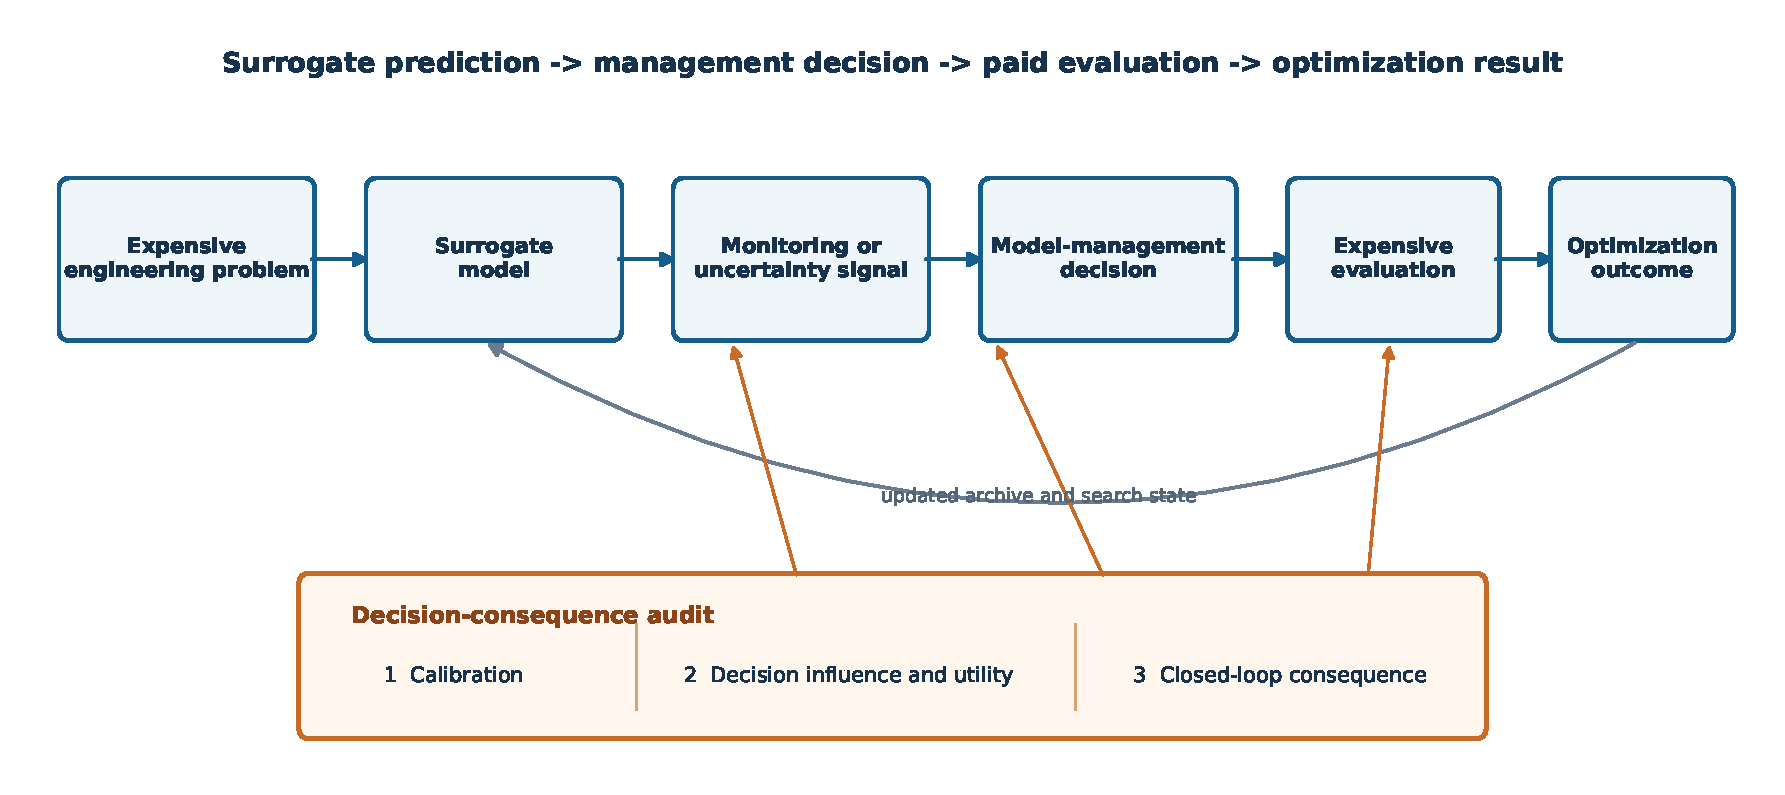
\includegraphics[width=\linewidth,height=.65\textheight,keepaspectratio]{figures/main_figure_1.pdf}
\caption{Decision-consequence auditing framework for surrogate-assisted optimization.}
\end{figure}

Figure 1 arranges the loop as six stages read from left to right: expensive engineering problem, surrogate model, monitoring or uncertainty signal, model-management decision, expensive evaluation and optimization outcome, with a return arrow that carries the updated archive and search state back to the surrogate model. Three annotation arrows connect the audit band beneath the chain to the stage each level interrogates, calibration to the monitoring signal, decision influence and utility to the model-management decision, and closed-loop consequence to the optimization outcome. Calibration therefore assesses the signal the optimizer encounters; decision analysis tests whether that signal changes a choice and improves common-state utility; closed-loop validation measures the final consequence after histories diverge.

\hypertarget{decision-pathways-and-ranking-invariance}{%
\subsection{Decision pathways and ranking invariance}\label{decision-pathways-and-ranking-invariance}}

A monitoring mechanism can affect optimization through candidate-specific ranking, an evaluation gate, a restart or stopping rule, a change of search region or population, or a stochastic exploration controller. The first audit step identifies at least one such path before additional expensive experiments are authorized.

\textbf{Lemma 1 (ranking invariance under a candidate-independent additive correction).} At evaluation t, suppose two rules receive an identical indexed candidate set, use deterministic and identical tie-breaking, and are evaluated in exact arithmetic. If every supported candidate shares the same additive correction \(c_t\), then minimizing \(H_t(x)=\mu_t(x)+c_t\) returns the same minimizer index as minimizing \(\mu_t(x)\).

\textbf{Proof.} For any indexed candidates \(x_i\) and \(x_j\), \(H_t(x_i)-H_t(x_j)=\mu_t(x_i)-\mu_t(x_j)\). Every strict comparison and exact tie is therefore preserved under the stated tie-breaking rule. The same indexed minimizer follows. $\square$

\textbf{Corollary 1.} If two configurations also share initialization, candidate generation, exploration decisions, all random streams and stochastic operators, numerical precision, and optimizer-state updates, and differ only by replacing the common-correction minimizer with the mean minimizer, their trajectories are identical by induction over evaluations. Finite-precision agreement is an implementation property and is checked separately in the experiment audit.

This result identifies a structural limitation of candidate-independent corrections; it does not invalidate uncertainty-aware surrogate management in general. Candidate-dependent posterior uncertainty, expected improvement, lower-confidence bounds, support-dependent rules, evaluation gates, restarts, and stopping policies may create decision paths that Lemma 1 does not remove.

\hypertarget{three-audit-levels-and-promotion-gate}{%
\subsection{Three audit levels and promotion gate}\label{three-audit-levels-and-promotion-gate}}

Common-history calibration fits the same frozen model and candidate pool, then evaluates monitoring losses and failures without updating the search. Common-state decision analysis compares the action with and without the mechanism at the same state; when actions differ, separate diagnostic labels measure true one-step utility. Independent closed-loop experiments then allow each policy to update its own history and evaluate final optimization behavior. One-step improvement diagnoses immediate exploitation value but is not a necessary condition for useful exploration. A lower immediate gain therefore identifies a need for delayed-value assessment rather than, by itself, grounds for stopping an exploration mechanism. The following procedure clarifies the interpretation of audit stages; it does not retrospectively alter any frozen experimental protocol or statistical comparison.

\textbf{Algorithm 1. Decision-consequence audit for a surrogate-assisted model-management mechanism.}

\textbf{Step 1 --- Specify.} Freeze the surrogate, candidate generator, monitoring signal, management or acquisition rule, expensive objective context, optimizer budget, audit-request budget, target horizon and margin, and deterministic replay information. In the independent conditional implementation, h0 is the first action and H=5 denotes five further common-rule actions. Output: protocol and information boundary.

\textbf{Step 2 --- Trace.} Follow the signal through ranking, evaluation, region, population, restart, stopping, or stochastic-exploration decisions. Gate: at least one candidate-dependent or otherwise actionable path.

\textbf{Step 3 --- Record and calibrate.} Persist every decision before its label. If the mechanism makes a calibrated-error claim, assess that claim on appropriately separated diagnostic data. Gate: an intact information boundary and evidence supporting the stated claim. Mechanisms that make no calibration claim are not required to pass a coverage test.

\textbf{Step 4 --- Test common-state utility.} Freeze optimization states and candidate pools, compare baseline and mechanism actions, and label only the prespecified diagnostic alternatives. Report decision-change frequency and immediate utility. For exploration, region, restart, or stopping mechanisms, prespecify a delayed-value assessment where needed. The implemented point-action intervention uses the same frozen training history, fitted kernel and first candidate pool, then the same declared continuation and candidate-seed stream with each branch updating its own history. For positive initial incumbent $m_{\mathrm{init}}$, the recorded conditional target is $d_j(H)=[m_0(H)-m_j(H)]/m_{\mathrm{init}}$, where $m_0$ is the baseline-branch incumbent. The primary implementation uses $H=5$ and margin $\tau=0.001$. Gate: an identifiable decision consequence and sufficient evidence to justify the next diagnostic expenditure; lower one-step improvement alone does not reject exploration.

\textbf{Step 5 --- Validate the closed loop.} Run independent optimization on held-out instances or engineering conditions under matched optimizer budgets, including when exploration requires a delayed-value test. Record diagnostic calls separately and include them in any deployment-cost comparison. Output: final objective consequence and total cost boundary.

\textbf{Step 6 --- Decide.} Promote, revise, stop, or retain an inconclusive decision using prespecified outcome tolerances and cost limits. Report the first unsupported claim and the evidence needed to resolve it. Promotion requires closed-loop evidence for the intended engineering use. Output: stage-wise audit record. The independent replay reports an exact branch alias, a measured target-horizon outcome, an h0 proxy, or an abstention because the target remains incomplete. For nonalias branches, better/tie/worse certification requires both baseline and alternative to reach h5; an immediate tie does not certify a later tie. Table~\ref{tab:review_contract} maps this implementation to its recorded inputs and outputs.

\Needspace{24\baselineskip}
\FloatBarrier\begingroup\fontsize{8.5}{10.5}\selectfont\setlength\tabcolsep{3pt}
\begin{longtable}{@{}>{\raggedright\arraybackslash}p{(\columnwidth - 4\tabcolsep) * \real{0.16}}>{\raggedright\arraybackslash}p{(\columnwidth - 4\tabcolsep) * \real{0.47}}>{\raggedright\arraybackslash}p{(\columnwidth - 4\tabcolsep) * \real{0.37}}@{}}
\caption{Implementation contract of the independent conditional audit. Values and information boundaries are taken from the frozen collection/replay code. This is a factual specification, not a new convergence result.}\label{tab:review_contract}\tabularnewline
\toprule
Object & Recorded implementation & Evidence boundary \\
\midrule
\endfirsthead
\toprule
Object & Recorded implementation & Evidence boundary \\
\midrule
\endhead
\bottomrule
\endlastfoot
Frozen state & Own 100-label history, fitted kernel, root candidate pool and first-action map & No alternative or probe response enters the frozen root fit \\
Continuation & Same declared mean or EI rule and candidate-seed stream; each branch updates its own history & The first action is the intervention; this target differs from whole-policy runs \\
Horizon & h0: first action; h5: five further common-rule actions & Six prefix requests per completed branch in this implementation \\
Target / margin & Baseline-minus-alternative final incumbent divided by initial incumbent; primary margin 0.001 & Better/tie/worse refers to the declared conditional h5 target \\
Branch reuse & Same history, fitted kernel, action, continuation, context and seed stream & A same-point response may be shared more broadly; an equal utility does not merge branches \\
Budget & Every branch-step request counts, including cache reads; primary B=18 & Not the number of additional physical attempts \\
Evidence output & Exact alias; measured h5 outcome; h0 proxy; budget-incomplete abstention & No partial trajectory certificate or general prediction guarantee \\
\end{longtable}
\endgroup


\Needspace{12\baselineskip}
\FloatBarrier\begingroup\fontsize{8.5}{10.5}\selectfont\setlength\tabcolsep{3pt}
\begin{longtable}{@{}>{\raggedright\arraybackslash}p{.17\linewidth}>{\raggedright\arraybackslash}p{\dimexpr.83\linewidth-2\tabcolsep\relax}@{}}
\caption{Frozen v1 conditional audit: executable operation specification. This table describes the existing code, including the unsuccessful adaptive heuristic; it does not propose a new optimizer. OpenAI Codex (GPT-6) assisted the code-to-method transcription.}\label{tab:conditional_algorithm}\tabularnewline
\toprule
Operation & Exact implementation \\
\midrule
\endfirsthead
\toprule
Operation & Exact implementation \\
\midrule
\endhead
\bottomrule
\endlastfoot
State / target & Freeze the 100-label history, fitted ARD kernel, first candidate pool, context and first actions. Baseline is the mean first action. Each branch updates its own history under the same mean or EI continuation and candidate-seed stream. $h0$ is the intervention; $H=5$ is five further actions. The primary target is $d_j=[m_0(5)-m_j(5)]/m_{\mathrm{init}}$, margin $\tau=0.001$. \\
Alias / access & Group exactly identical first actions only within the same state and declared continuation. If $K=1$, output structural tie for all names with zero requests. Otherwise \texttt{observe(branch,step)} may reveal only the next prefix response. Each request costs one, including an exact cache read. \\
Fixed depth & Complete the baseline to step 5; then complete alternatives in original class order while budget remains. Original class insertion follows mean, EI, PI, LCB. Incomplete comparisons abstain. Full mode uses $6K$ requests as its allowance. \\
Breadth / proxy & Breadth loops over steps 0--5 and advances baseline then alternatives at each step. Immediate mode reads h0 for each class; its labels are proxies for the h5 target, not certificates. \\
Adaptive reads & Read h0 and h1 for all classes, baseline first; then complete the baseline. Rank alternatives by descending $p_j=|m_0(1)-m_j(1)|/m_{\mathrm{init}}+\sigma_j^{\mathrm{root}}/m_{\mathrm{init}}$. Equal priorities use original class order. Advance each alternative to stages 3 and 5 before moving to the next. This priority is an observed-effect/uncertainty heuristic, not a confidence bound. \\
Measured outputs & A nonalias better/tie/worse certificate requires both baseline and alternative to reach h5. Use better if $d_j>\tau$, worse if $d_j<-\tau$, otherwise tie. Budget-incomplete output is abstain; an immediate tie never certifies a later tie. \\
Acquisitions & Independent budget collection uses 1024 candidates, normalized targets, $\alpha=10^{-6}$ and $\kappa=2$. EI/PI use an improvement margin $0.05$ times training-label standard deviation. ARD parameters are fitted once at the shared 50-label warm state (max 30 iterations), then fixed. These settings differ from the archived intervention and transfer studies. \\
Calibration proxy & Eight frozen-root probes give NRMSE (scaled by training-label standard deviation) and empirical coverage of $\mu\pm1.6448536269514722\sigma$. The constructed gate requires NRMSE $\leq0.25$ and coverage $\geq0.8$. If eligible, classify the root-EI difference divided by $m_{\mathrm{init}}$ using the same margin; otherwise abstain. It predicts h5 utility without a horizon guarantee. The original comparator charges eight probes in all 30 states. \\
State selection & Start with mean and effect threshold $\tau$. Visit EI, PI, LCB; replace the selected control only for label better and a strictly larger recorded effect. Thus exact ties retain the earlier control. Select only from the disclosed outputs, not oracle h5 truth. \\
Loss / averaging & State-selection loss is $100[m_{\mathrm{selected}}(5)-\min_j m_j(5)]/m_{\mathrm{init}}$. Average over all 30 states, including alias-only states. Complete truth is used only after the reader finishes, to evaluate the decision; it cannot change the observation trace. Ten shared seed blocks, not these dependent states or contrasts, are the independent units. \\
\end{longtable}
\endgroup



The framework can return a positive result, and does so on recorded data. Classical GP acquisition is a candidate-dependent positive control because both its predicted improvement and its uncertainty vary across candidates, so it can change ranking and passes the structural decision-influence check; passing that first check does not guarantee superior endpoints, it authorizes empirical utility and closed-loop evaluation. Section 6.4 applies a declared promotion rule to the three recorded acquisition rules and reports one promotion, one stop and one held-for-revision verdict.

\hypertarget{diagnostic-cost-and-scope-of-deployment-claims}{%
\subsection{Diagnostic cost and scope of deployment claims}\label{diagnostic-cost-and-scope-of-deployment-claims}}

The optimization budget and the audit budget are different quantities. The total physical-call cost includes additional optimizer evaluations, additional diagnostic evaluations, and recovery or verification calls; previously paid deterministic labels reused from an archive are identified separately. A comparison of optimizer endpoints at equal budgets does not establish that the audit itself saves evaluations. In the independent replay, each branch-step request is charged, including a cache read; a completed branch needs $H+1=6$ requests. Its primary budget 18 is per state. For $K$ exact branch classes, full-baseline/full-alternative reporting can complete at most $\min(K-1,\max(0,\lfloor B/(H+1)\rfloor-1))$ nonbaseline comparisons under this request contract. This elementary capacity does not bound additional physical solves or audits with a justified early certificate.

The independent internal validation uses 907,200 optimization evaluations and 1,990,656 additional diagnostic labels. Those full-pool diagnostics support mechanism analysis on inexpensive benchmark functions, but are not proposed as the default screening cost for expensive engineering simulations. A bounded engineering audit should prespecify states, label the union of selected alternatives where possible, and stop or report inconclusive when its diagnostic limit is reached. Any claim of net savings must compare the audited workflow with a prespecified unaudited workflow, including diagnostic overhead. Section 6.5 reports a complete paid-workflow comparison with endpoint losses; it does not establish performance-preserving net savings.

\hypertarget{decision-equivalence-and-the-minimum-immediate-diagnostic-budget}{%
\subsection{Decision equivalence and the minimum immediate diagnostic budget}\label{decision-equivalence-and-the-minimum-immediate-diagnostic-budget}}

For a frozen state \(s\), let \(a_j(s)\) be the exact point selected by policy j and let \(c\) identify the deterministic objective context: simulator, physical condition, parameterization, and numerical configuration. Policies are immediately decision-equivalent when they select the same bitwise point under the same \(c\). This is a local relation. Equivalent first actions do not make later policies equivalent, and labels must not be reused across changed physical conditions or noisy objectives without an additional justification. Whole conditional branches share a record only when the frozen history, fitted kernel, first action, objective context, continuation and deterministic seed stream also coincide; across other states, exact point/context equality permits response reuse only. The reported implementations evaluate point-acquisition rules; conditional restart, region and stopping interventions are not independently validated here.

Let \(X\) be the union of distinct context-point pairs selected by all prespecified states and policies, and let \(A\) contain the exact responses that the auditor is permitted to reuse after decisions have been frozen. For incumbent \(m_s\) and fixed positive scale \(v_s\), the reported immediate utility is \(u_j(s)=\max(0,m_s-f_c(a_j(s)))/v_s\). The additional deterministic query requirement is

\[N_{\mathrm{diag}}=|X\setminus A|.\]

\textbf{Proposition 1 (minimum worst-case immediate diagnostic queries).} Suppose the objective is an unrestricted deterministic oracle, all selected points and incumbents are frozen, and each unqueried response can independently lie on either side of at least one associated incumbent while all other responses remain fixed. Querying each member of \(X\) outside \(A\) once suffices to report every immediate utility. In the worst case, fewer queries cannot determine all utilities exactly.

\textbf{Proof.} Sufficiency follows by assigning the same exact response to every context-point equivalence class and reusing only permitted responses. For necessity, consider an unqueried member \(x\) in a class with incumbent \(m\). Two objectives can agree on all available and queried responses while taking values \(m-\delta\) and \(m+\delta\) at \(x\) for \(\delta>0\) (\(\delta<m\) for a positive objective); the resulting utilities differ. No procedure using only those shared observations can distinguish them. For a finite set of distinct points, disjoint smooth local interpolants can realize these assignments, so smoothness alone does not remove the ambiguity. Querying each undetermined member resolves it. A certified response bound or a restricted physical objective class may reduce this worst-case requirement; no such additional exact inference is used here. $\square$

The proposition is an allocation rule for a specified exact diagnostic report, not a lower bound on all possible optimization audits. It does not prove that the queries improve search. Section 6.3 illustrates both the within-state equivalence reduction and the additional reduction from permitted source-response and diagnostic-cache reuse. The source label at a frozen original action is consulted only after the intervention choices are fixed; it never enters the predecision GP fit. All thresholds for a deployment decision must still be fixed for the intended engineering use before its validation outcomes are observed. The added transfer study supplies descriptive evidence, not a retrospectively chosen promotion threshold.

\hypertarget{experimental-design}{%
\section{Experimental Design}\label{experimental-design}}

\hypertarget{representative-monitored-optimizer-and-search-framework}{%
\subsection{Representative monitored optimizer and search framework}\label{representative-monitored-optimizer-and-search-framework}}

A temporal residual monitor is used as the representative audited mechanism. For a selected point x\_\allowbreak t, the standardized signed residual is r\_\allowbreak t={[}y\_\allowbreak t-mu\_\allowbreak t(x\_\allowbreak t){]}/s\_\allowbreak t, where s\_\allowbreak t is the standard deviation of the current training labels and is replaced by one if it is zero. Historical residuals retain their prediction-time models and scales. For candidate x, the monitor forms H\_\allowbreak t(x)=mu\_\allowbreak t(x)+s\_\allowbreak t q\_\allowbreak t(x), where q\_\allowbreak t(x) is the nonnegative weighted 0.9 quantile of at most the latest 100 residuals. Temporal weights have a half-life of 25 evaluations; spatial variants use a Gaussian kernel and an effective-sample-size support guard of 20.

The temporal prototype PEM-T converts recent failures, normalized bound width, and evaluations without incumbent improvement into an exploration probability between 0.1 and 0.8. Exploration selects the candidate with the largest minimum distance to the archive. Otherwise, the smallest supported upper value is used when an improvement declaration is available and the monitor is not alarmed; the smallest predicted mean is used in the remaining cases. fixed 0.1 retains the same model and candidate process with exploration probability 0.1. Under the temporal bound, q\_\allowbreak t and s\_\allowbreak t are common to supported candidates, so Lemma 1 predicts that the upper-value and mean exploitation rankings coincide.

The internal optimizer uses a randomized Latin hypercube with 2D+20 initialization points. The first D+10 points train the initial model; the remaining D+10 are predicted before labeling and create startup residuals. Inputs are scaled to the unit cube. A regularized Gaussian radial-basis-function surrogate uses distance divided by the square root of D, length scale 0.25, ridge 10\^{}-6, and standardized labels. At most 256 observations are retained through an elite-plus-farthest-point rule.

Each iteration proposes 256 candidates: 128 reflected differential-evolution proposals and 128 scrambled Sobol points. Duplicates and candidates within 10\^{}-10 of evaluated points are replaced. Purpose-specific random streams depend on seed and evaluation index rather than the total budget.

\hypertarget{development-and-independent-validation}{%
\subsection{Development and independent validation}\label{development-and-independent-validation}}

Development uses eight prespecified Black-Box Optimization Benchmarking (BBOB) functions, dimensions 10 and 20, instances 1-3, and three repeats. Thirteen internal configurations separate exploration, residual weighting, and feedback components. The budget is 10D. The required gate compares PEM-T with a fixed exploration control selected only within the development protocol. Failure of the gate prevents any optimization-superiority claim.

After the gate fails, the unchanged mechanism is frozen on all 24 noiseless BBOB functions, dimensions 10, 20, and 40, instances 11-13, and three repeats. Six internal configurations produce 3,888 runs and 907,200 paid evaluations. Three history policies produce 7,776 frozen states and 1,990,656 diagnostic labels. Development and validation estimates are never pooled.

The endpoint is the base-10 logarithm of final error relative to common initialization error, with numerical flooring at 10\^{}-12. Repeats are summarized within function-instance cells, instances are averaged, and functions receive equal weight. Nine prespecified validation contrasts form one Holm family. Paired hierarchical bootstrap intervals resample functions, instances, and common repeat indices. These intervals summarize suite heterogeneity and are not presented as a population theorem for all black-box tasks.

\hypertarget{external-and-application-evidence}{%
\subsection{External and application evidence}\label{external-and-application-evidence}}

Sobol, CMA-ES, classical GP expected improvement, and author-code TuRBO-1 provide budget-matched descriptive references \citep{ref25}. They retain their own initialization and search mechanisms, so these comparisons are not same-history causal effects. In the finite-element application, GP expected improvement (GP-EI), probability of improvement (GP-PI), and the lower-confidence-bound form of GP-UCB are additionally run from the same initial observations as the internal methods. All three acquisitions use the same Matérn-5/2 Gaussian process, candidate pool, and local-search budget; GP-PI uses a margin equal to 0.01 times the observed response standard deviation, and GP-UCB uses a fixed confidence multiplier of 2.0. DRSO uses the authors' public relation-model-assisted evolutionary implementation at commit 03c19d4 \citep{ref30}. The population size is set to 58 solely to accept the common initial archive; its relation models, unevaluated-population update, reproduction, training cap, and remaining defaults are unchanged. Three LassoBench tasks provide application transfer under fixed data and splits \citep{ref24}. The BBOB implementation and reporting follow the COCO comparison framework \citep{ref26}. Complete tables, the 300-dimensional extension, resource measurements, sensitivity studies, interruption accounting, and file-level audits appear in the Supplementary Materials.

\hypertarget{mechanism-results}{%
\section{Mechanism Results}\label{mechanism-results}}

\hypertarget{development-gate-and-implementation-invariants}{%
\subsection{Development gate and implementation invariants}\label{development-gate-and-implementation-invariants}}

All 1,872 development optimization runs and 432 common-history runs complete without exceptions. PEM-T and the configuration that removes its upper-value mode have identical trajectories in all 144 matched pairs. Temporal monitoring with fixed 0.3 management likewise matches fixed 0.3 mixing in all 144 pairs. These are implementation confirmations of Lemma 1 and Corollary 1, rather than independent effective components.

The development-selected control is fixed 0.1. PEM-T is worse on all eight development functions in both dimensions. Its function-weighted log-relative endpoint difference is +0.2831 in D=10 and +0.1810 in D=20, where positive values favor fixed 0.1. The required optimization-benefit gate is therefore unmet before the independent validation begins.

\hypertarget{independent-endpoint-and-immediate-decision-effects}{%
\subsection{Independent endpoint and immediate decision effects}\label{independent-endpoint-and-immediate-decision-effects}}

Table~\ref{tab:validation} reports the nine prespecified validation comparisons. PEM-T increases final relative error in all three dimensions. The base-10 differences correspond to geometric error ratios of 1.468, 1.258, and 1.159 for dimensions 10, 20, and 40. The effect decreases with dimension but remains in the unfavorable direction for 60 of 72 function-level comparisons. Common-state feedback decisions also have lower true immediate improvement than mean-greedy decisions in every dimension.

\FloatBarrier\begingroup\fontsize{8.5}{10.5}\selectfont\setlength\tabcolsep{3pt}

\begin{longtable}[]{@{}
  >{\raggedleft\arraybackslash}p{(\columnwidth - 10\tabcolsep) * \real{0.1667}}
  >{\raggedright\arraybackslash}p{(\columnwidth - 10\tabcolsep) * \real{0.1667}}
  >{\raggedleft\arraybackslash}p{(\columnwidth - 10\tabcolsep) * \real{0.1667}}
  >{\raggedleft\arraybackslash}p{(\columnwidth - 10\tabcolsep) * \real{0.1667}}
  >{\raggedleft\arraybackslash}p{(\columnwidth - 10\tabcolsep) * \real{0.1667}}
  >{\raggedleft\arraybackslash}p{(\columnwidth - 10\tabcolsep) * \real{0.1667}}@{}}
\caption{Prespecified independent validation contrasts. Endpoint values above zero favor fixed 0.1; immediate values below zero favor mean-greedy selection. History-interaction values are selected-point minus pool failure differences, so positive values mean the policy's selected points fail more often than its own candidate pool. Direction counts give positive and negative repeat-level outcomes; the denominator is 24 for the endpoint and history-interaction rows and 19, 21 and 21 for the immediate-improvement rows, where exact ties are excluded.}\label{tab:validation}\tabularnewline
\toprule\noalign{}
\begin{minipage}[b]{\linewidth}\raggedleft
Dimension
\end{minipage} & \begin{minipage}[b]{\linewidth}\raggedright
Contrast
\end{minipage} & \begin{minipage}[b]{\linewidth}\raggedleft
Estimate
\end{minipage} & \begin{minipage}[b]{\linewidth}\raggedleft
95\% bootstrap interval
\end{minipage} & \begin{minipage}[b]{\linewidth}\raggedleft
Direction count
\end{minipage} & \begin{minipage}[b]{\linewidth}\raggedleft
Holm p
\end{minipage} \\
\midrule\noalign{}
\endfirsthead
\toprule\noalign{}
\begin{minipage}[b]{\linewidth}\raggedleft
Dimension
\end{minipage} & \begin{minipage}[b]{\linewidth}\raggedright
Contrast
\end{minipage} & \begin{minipage}[b]{\linewidth}\raggedleft
Estimate
\end{minipage} & \begin{minipage}[b]{\linewidth}\raggedleft
95\% bootstrap interval
\end{minipage} & \begin{minipage}[b]{\linewidth}\raggedleft
Direction count
\end{minipage} & \begin{minipage}[b]{\linewidth}\raggedleft
Holm p
\end{minipage} \\
\midrule\noalign{}
\endhead
\bottomrule\noalign{}
\endlastfoot
10 & PEM-T minus fixed 0.1 endpoint & 0.1668 & {[}0.0749, 0.2391{]} & 22 positive, 2 negative & 5.36e-6 \\
20 & PEM-T minus fixed 0.1 endpoint & 0.0998 & {[}0.0467, 0.1905{]} & 19 positive, 5 negative & 0.00170 \\
40 & PEM-T minus fixed 0.1 endpoint & 0.0639 & {[}0.0130, 0.1123{]} & 19 positive, 5 negative & 0.00170 \\
10 & History interaction (selected minus pool failure) & 0.0851 & {[}0.0311, 0.1234{]} & 20 positive, 4 negative & 0.00149 \\
20 & History interaction (selected minus pool failure) & 0.1225 & {[}0.0696, 0.1948{]} & 21 positive, 3 negative & 0.00065 \\
40 & History interaction (selected minus pool failure) & 0.1449 & {[}0.0941, 0.2244{]} & 17 positive, 7 negative & 0.00170 \\
10 & Feedback minus mean immediate improvement & -0.0170 & {[}-0.0431, -0.0067{]} & 1 positive, 18 negative & 0.00078 \\
20 & Feedback minus mean immediate improvement & -0.0158 & {[}-0.0352, -0.0079{]} & 0 positive, 21 negative & 0.00048 \\
40 & Feedback minus mean immediate improvement & -0.0344 & {[}-0.0630, -0.0100{]} & 1 positive, 20 negative & 0.00048 \\
\end{longtable}

\endgroup

The function-level distribution underlying the aggregate endpoint contrasts is shown in Figure 2.

\begin{figure}
\centering
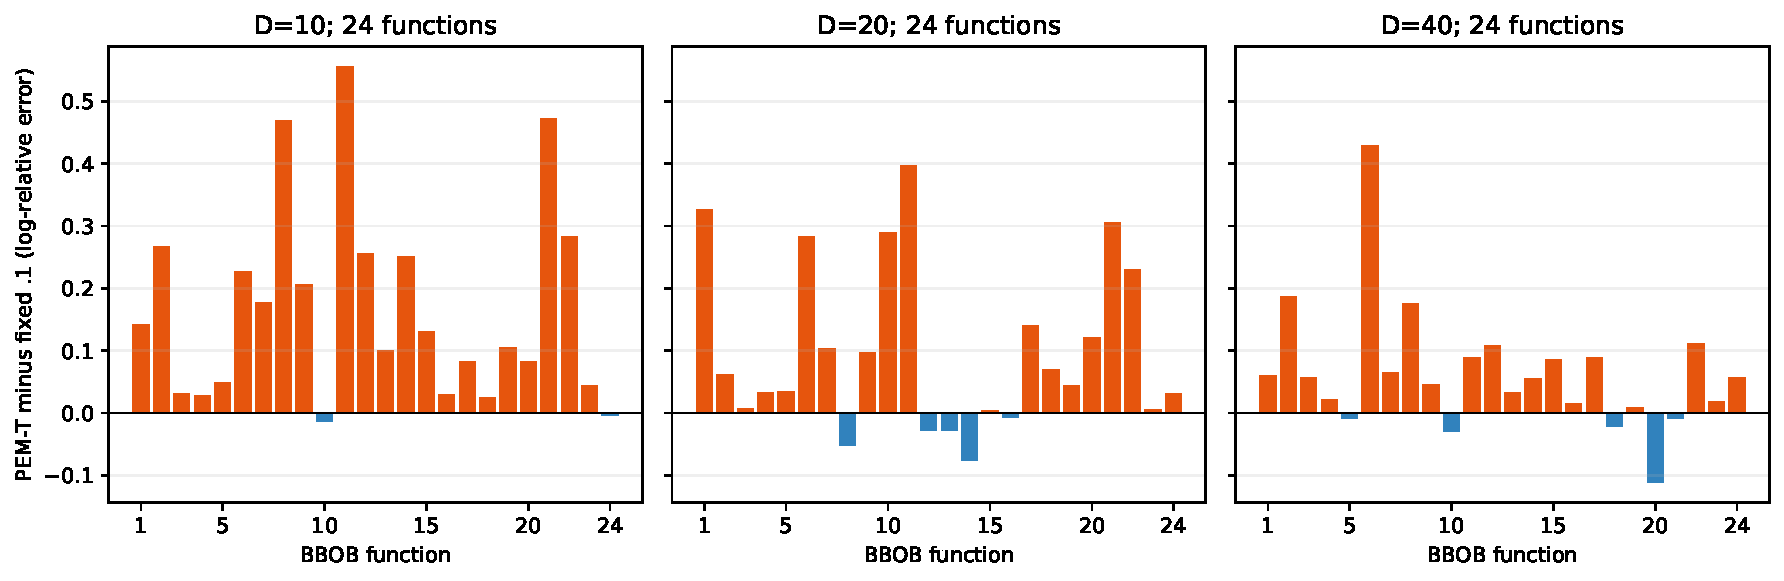
\includegraphics[width=\linewidth,height=.65\textheight,keepaspectratio]{figures/main_figure_2.pdf}
\caption{Function-level endpoint effects in the independent BBOB validation. Positive values indicate larger PEM-T errors.}
\end{figure}

Figure 2 displays all 24 function-level effects separately for each dimension rather than only the suite average. Each panel covers functions 1 to 24 on the horizontal axis against the difference in base-10 log-relative error on the vertical axis; bars above the zero line are drawn in orange and the few below it in blue. Most bars lie above the zero line: 22 of 24 in dimension 10 and 19 of 24 in both dimensions 20 and 40. The few negative bars show that the result is not pointwise uniform, while the shrinking bar heights across panels agree with the smaller aggregate effect at higher dimension. The conclusion is therefore based on a broad directional pattern with disclosed exceptions, not on one dominant benchmark function.

\hypertarget{calibration-does-not-identify-optimization-utility}{%
\subsection{Calibration does not identify optimization utility}\label{calibration-does-not-identify-optimization-utility}}

PEM-T explores 39.7\%, 36.4\%, and 34.4\% of post-initialization evaluations in dimensions 10, 20, and 40, compared with approximately 10\% for fixed 0.1. Its observed selected-point upper-bound failure fractions are 0.1008, 0.0942, and 0.0964, close to the nominal monitoring level. Nevertheless, its endpoints and common-state decisions are worse. A near-target aggregate failure fraction therefore does not imply efficient budget allocation.

Improvement declarations provide a second example. PEM-T makes 31, 34, and 155 declarations across the three dimensions; 20, 27, and 30 are false. The corresponding pooled false-declaration fractions are 0.645, 0.794, and 0.194. A one-sided failure rate near 0.1 cannot control the conditional error among the small subset declared to improve the incumbent.

History also changes the object being monitored. Under fixed 0.3 mixing, selected-point failures exceed pool failures, whereas under greedy histories the relationship reverses. The prespecified interaction is positive in all three dimensions and passes Holm adjustment. Selection-induced differences should therefore be attributed to the coupled history and policy, not treated as a universal direction of undercoverage.

The reversal of selected-point and pool failure differences across frozen history policies is shown in Figure 3.

\begin{figure}
\centering
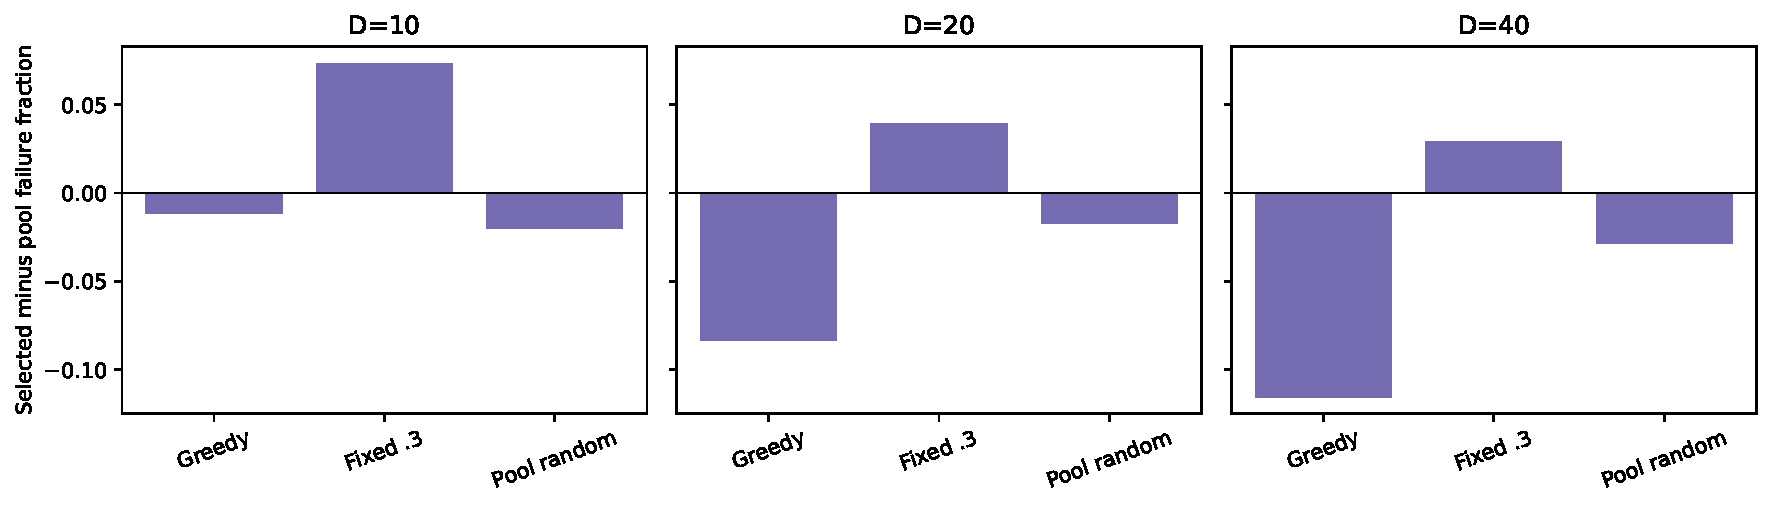
\includegraphics[width=\linewidth,height=.65\textheight,keepaspectratio]{figures/main_figure_3.pdf}
\caption{Selected-point minus pool failure differences under frozen history policies.}
\end{figure}

Figure 3 makes the history dependence visible. Each panel, one per dimension, plots the selected-point minus pool failure fraction on the vertical axis for the three frozen history policies on the horizontal axis, and the zero line marks identical failure fractions for the two monitored objects. Fixed 0.3 histories place the selected-point failure fraction above the pool value in all three dimensions, whereas greedy histories place it below the pool value. Random-pool histories remain closer to zero and are negative in each panel. Because the sign changes with the policy that generated the frozen state, a single universal ``selection penalty'\,' would misrepresent the monitored process.

Spatial-temporal weighting lowers selected-point quantile loss in the prespecified diagnostic comparisons, yet its closed-loop endpoint remains worse than fixed 0.1 in each dimension. This is the central empirical separation: a better residual estimate can still direct evaluations toward candidates with low optimization value.

To isolate the evidential role of each audit stage, a stage-omission ablation is constructed from the frozen records. Unlike an optimizer-component ablation, omitting an audit stage does not alter the evaluated trajectory; it removes the corresponding basis for inference. Table~\ref{tab:stage_ablation} states the strongest conclusion still supported at each stopping point and the evidence that would be lost.

\FloatBarrier\begingroup\fontsize{8.5}{10.5}\selectfont\setlength\tabcolsep{3pt}

\begin{longtable}[]{@{}
  >{\raggedright\arraybackslash}p{(\columnwidth - 4\tabcolsep) * \real{0.3333}}
  >{\raggedright\arraybackslash}p{(\columnwidth - 4\tabcolsep) * \real{0.3333}}
  >{\raggedright\arraybackslash}p{(\columnwidth - 4\tabcolsep) * \real{0.3333}}@{}}
\caption{Stage-omission ablation and the resulting loss of evidence.}\label{tab:stage_ablation}\tabularnewline
\toprule\noalign{}
\begin{minipage}[b]{\linewidth}\raggedright
Available audit evidence
\end{minipage} & \begin{minipage}[b]{\linewidth}\raggedright
Apparent conclusion for the representative monitor
\end{minipage} & \begin{minipage}[b]{\linewidth}\raggedright
Information lost if the audit stops here
\end{minipage} \\
\midrule\noalign{}
\endfirsthead
\toprule\noalign{}
\begin{minipage}[b]{\linewidth}\raggedright
Available audit evidence
\end{minipage} & \begin{minipage}[b]{\linewidth}\raggedright
Apparent conclusion for the representative monitor
\end{minipage} & \begin{minipage}[b]{\linewidth}\raggedright
Information lost if the audit stops here
\end{minipage} \\
\midrule\noalign{}
\endhead
\bottomrule\noalign{}
\endlastfoot
Calibration only & Selected-point failure is close to 0.1 and may appear satisfactory. & No evidence that exploitation ranking changes or that selected actions are useful. \\
Calibration plus ordering analysis & The temporal additive correction is exploitation-redundant; feedback can act through exploration. & The utility of the changed exploration decisions remains unknown. \\
Ordering plus common-state utility & Feedback changes actions, but those actions have lower immediate improvement than mean-greedy choices. & Delayed effects after histories diverge remain untested. \\
Full audit including closed loop & The controller does not pass the held-out optimization-benefit gate under the tested budgets. & No omitted audit stage is used to claim deployment value. \\
\end{longtable}

\endgroup

This evidence ablation uses the same frozen results rather than rerunning a modified optimizer because the ablated objects are inferential stages rather than search operators. It shows why a calibration-only assessment would have produced an incomplete reliability conclusion, why algebraic pathway analysis can identify redundancy without additional objective calls, and why common-state and closed-loop evidence answer distinct questions.

\hypertarget{engineering-application-surrogate-assisted-structural-optimization}{%
\section{Engineering Application: Surrogate-Assisted Structural Optimization}\label{engineering-application-surrogate-assisted-structural-optimization}}

\hypertarget{problem-and-parameterization}{%
\subsection{Problem and parameterization}\label{problem-and-parameterization}}

EngiBench Beams2D v1 supplies a density-based finite-element model of the right half of a symmetric Messerschmitt-Bolkow-Blohm beam \citep{ref23}. Surrogate-assisted evolutionary optimization has previously been developed for expensive structural design \citep{ref18}, and uncertainty-guided reliable-region search has been studied for expensive engineering optimization \citep{ref35}. Here, the beam provides engineering application validation of the audit framework within an expensive structural optimization workflow. The domain uses 100 by 50 bilinear elements. Horizontal degrees of freedom along the left symmetry boundary are fixed, the lower-right vertical degree of freedom is supported, and a unit downward load is applied at the top-left of the modeled half-beam. The material interpolation uses minimum stiffness 10\^{}-9, unit maximum stiffness, penalization power 3, and Poisson ratio 0.3. The objective is structural compliance; lower values are better.

Direct optimization of all 5,000 element densities is outside the studied surrogate's budget and initialization regime. A constrained engineering family is defined in which 19 effective logits plus one fixed anchor form a 4 by 5 coarse field. Cubic interpolation expands the field to 50 by 100 elements. A scalar logistic shift is solved by bisection so that every design has mean density 0.35. The study therefore evaluates model management within this smooth 19-dimensional design family rather than claiming general topology-optimization performance.

\hypertarget{application-protocol-and-audit-results}{%
\subsection{Application protocol and audit results}\label{application-protocol-and-audit-results}}

Before formal labels, five methods, ten repeats, and 200 evaluations per run are frozen. The first batch keeps the native 38-point initialization of GP-EI and TuRBO-1 while Greedy, fixed 0.1, and PEM-T share a 58-point initialization. A prespecified sensitivity batch then reruns GP-EI and TuRBO-1 from exactly the same 58 points and deterministic labels as the internal methods. Two acquisition controls, GP-PI and GP-UCB, and the author-code DRSO SAEA are subsequently run from the same archive. Their subsequent searches retain their stated acquisition, trust-region, relation-model, evolutionary, and candidate-generation rules. The original 50 trajectories contain 10,000 paid finite-element evaluations. The five shared-initialization external controls add 10,000 algorithm-budget observations, reuse 2,900 initial labels, and make 7,100 additional finite-element calls. All 100 trajectories finish without failure or exact duplicate points. Independent endpoint diagnostics reproduce the original GP-EI and TuRBO-1 sensitivity endpoints within a maximum relative difference of 6.23e-12; event-level audits accept every GP-PI, GP-UCB, and DRSO trajectory.

\FloatBarrier\begingroup\fontsize{8.5}{10.5}\selectfont\setlength\tabcolsep{3pt}

\begin{longtable}[]{@{}
  >{\raggedright\arraybackslash}p{(\columnwidth - 8\tabcolsep) * \real{0.2000}}
  >{\raggedleft\arraybackslash}p{(\columnwidth - 8\tabcolsep) * \real{0.2000}}
  >{\raggedleft\arraybackslash}p{(\columnwidth - 8\tabcolsep) * \real{0.2000}}
  >{\raggedleft\arraybackslash}p{(\columnwidth - 8\tabcolsep) * \real{0.2000}}
  >{\raggedleft\arraybackslash}p{(\columnwidth - 8\tabcolsep) * \real{0.2000}}@{}}
\caption{Finite-element endpoint compliance over ten optimization repeats.}\label{tab:beam_endpoints}\tabularnewline
\toprule\noalign{}
\begin{minipage}[b]{\linewidth}\raggedright
Method
\end{minipage} & \begin{minipage}[b]{\linewidth}\raggedleft
Median
\end{minipage} & \begin{minipage}[b]{\linewidth}\raggedleft
Q1
\end{minipage} & \begin{minipage}[b]{\linewidth}\raggedleft
Q3
\end{minipage} & \begin{minipage}[b]{\linewidth}\raggedleft
Median improvement after shared initialization
\end{minipage} \\
\midrule\noalign{}
\endfirsthead
\toprule\noalign{}
\begin{minipage}[b]{\linewidth}\raggedright
Method
\end{minipage} & \begin{minipage}[b]{\linewidth}\raggedleft
Median
\end{minipage} & \begin{minipage}[b]{\linewidth}\raggedleft
Q1
\end{minipage} & \begin{minipage}[b]{\linewidth}\raggedleft
Q3
\end{minipage} & \begin{minipage}[b]{\linewidth}\raggedleft
Median improvement after shared initialization
\end{minipage} \\
\midrule\noalign{}
\endhead
\bottomrule\noalign{}
\endlastfoot
Greedy & 1445.1 & 1300.8 & 1694.9 & 0.362 \\
fixed 0.1 & 1435.6 & 1354.2 & 1580.7 & 0.383 \\
PEM-T & 1972.8 & 1759.3 & 2168.9 & 0.251 \\
GP-EI & 2308.5 & 1989.4 & 2464.5 & 0.000 \\
GP-PI & 1233.1 & 921.2 & 1399.7 & 0.517 \\
GP-UCB & 2308.7 & 2223.8 & 2827.3 & 0.000 \\
DRSO & 647.4 & 580.4 & 780.0 & 0.747 \\
TuRBO-1 & 574.0 & 534.7 & 665.3 & 0.751 \\
\end{longtable}

\endgroup

PEM-T minus fixed 0.1 has median paired compliance difference +488.7, with interquartile range +134.7 to +814.7; PEM-T is better in two repeats and worse in eight. The corresponding comparison with greedy has median difference +575.2 and the same direction count. These and the following differences are medians of the ten repeat-matched endpoint differences, not differences between the medians in Table~\ref{tab:beam_endpoints}. These and the following differences are medians of the ten repeat-matched endpoint differences, not differences between the medians in Table~\ref{tab:beam_endpoints}; the repeat-level endpoints belong to the prespecified application runs and are not included in the released tree. Under matched initialization, GP-EI minus PEM-T has median difference +242.8; GP-EI is better once, tied three times, and worse six times (paired Wilcoxon Holm-adjusted p=0.0469). Within the three added-control family, GP-PI minus PEM-T has median difference -876.1 and nine wins (Holm-adjusted p=0.0117), GP-UCB has median difference +574.6 with two wins, two ties, and six losses (p=0.0391), and DRSO has median difference -1334.6 with nine wins and one loss (p=0.0117). TuRBO-1 minus PEM-T has median difference -1372.3 and is better in all ten repeats (Holm-adjusted p=0.00391 in the original sensitivity family). Changing from native to shared initialization produces no supported endpoint shift for GP-EI (Holm-adjusted p=0.320) or TuRBO-1 (p=0.695). The application therefore distinguishes a weak acquisition setting from successful Bayesian, evolutionary-surrogate, and trust-region controls under the same starting evidence.

The shared-initialization finite-element trajectories and their between-repeat dispersion are shown in Figure 4.

\begin{figure}
\centering
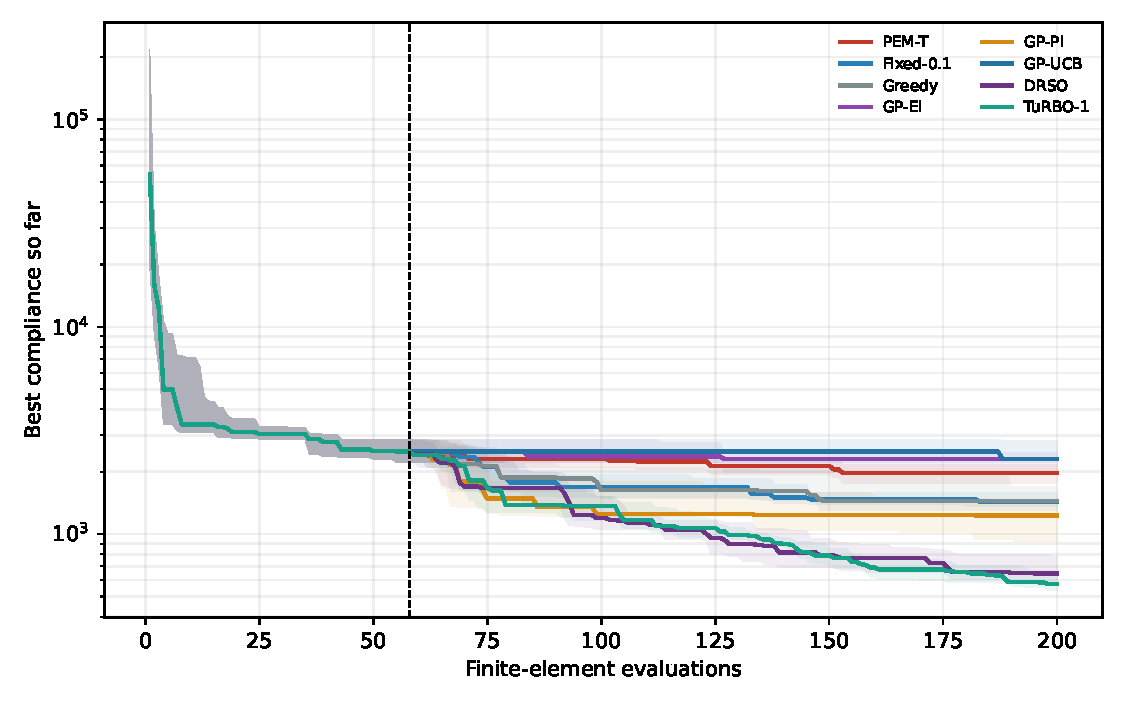
\includegraphics[width=\linewidth,height=.65\textheight,keepaspectratio]{figures/main_figure_4.pdf}
\caption{Median and interquartile best-so-far finite-element compliance under a shared 58-point initialization; the dashed line marks the end of initialization.}
\end{figure}

Figure 4 separates the common initialization from method-specific search. Best compliance so far is plotted on a logarithmic vertical axis spanning 10\^{}3 to 10\^{}5, the horizontal axis counts finite-element evaluations up to 200, and the dashed vertical line marks the end of the 58-point initialization. One curve and one shaded interquartile band are drawn for each of the eight methods; the control is labelled Fixed-0.1 in the legend. All curves share the same values up to the dashed boundary. TuRBO-1 and DRSO then improve rapidly and reach the lowest endpoint group. GP-PI also produces sustained improvement and finishes below the three internal methods, whereas GP-EI and GP-UCB show little median improvement after initialization. Greedy and fixed 0.1 improve more gradually and remain below PEM-T near the endpoint. The shaded interquartile bands preserve between-repeat variability and show that the endpoint ordering is not produced by a single trajectory.

Representative endpoint density fields for all eight shared-initialization methods are shown on the common material-density scale in Figure 5.

\begin{figure}
\centering
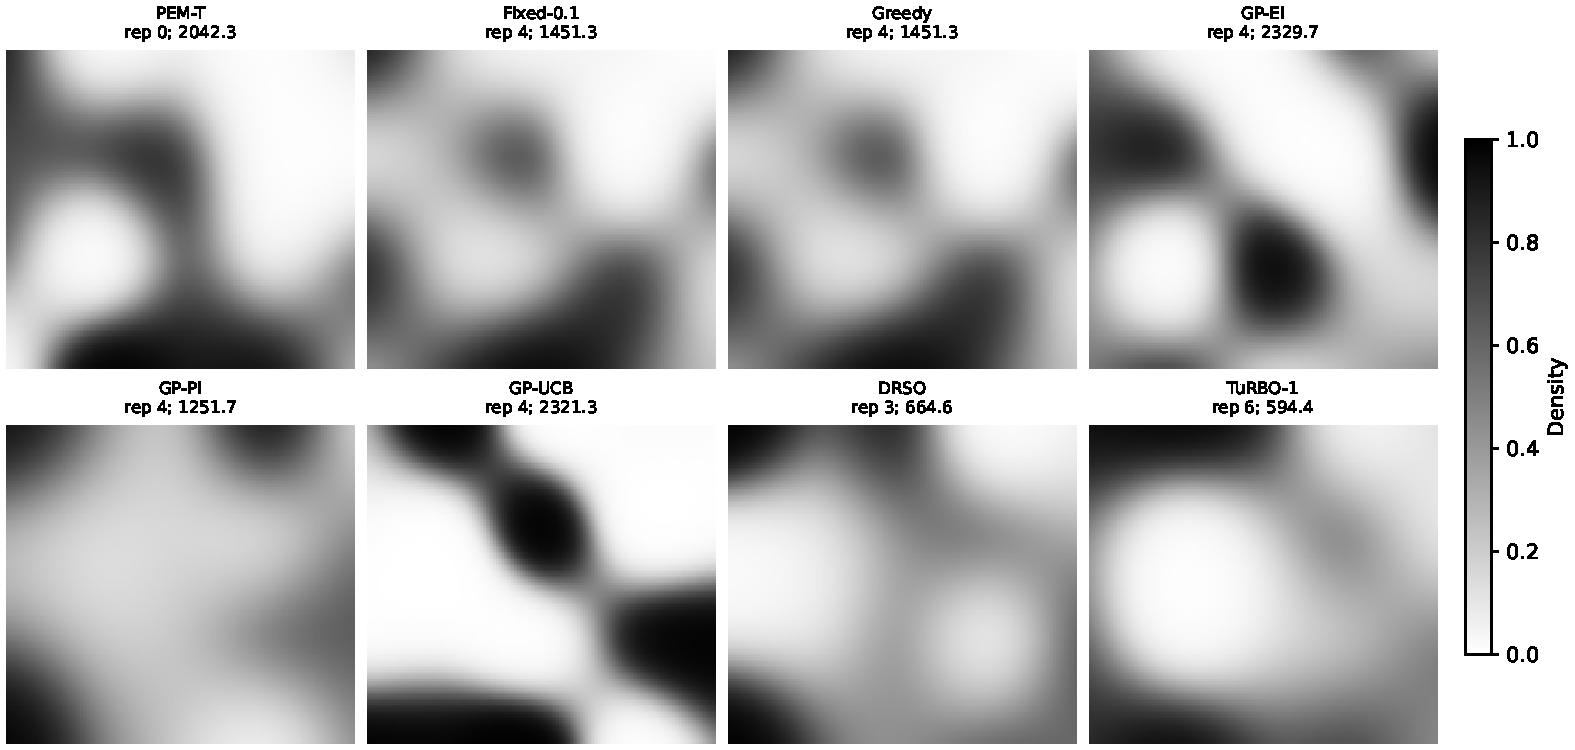
\includegraphics[width=\linewidth,height=.65\textheight,keepaspectratio]{figures/main_figure_5.pdf}
\caption{Representative median-run density fields for all eight methods under the shared-initialization comparison.}
\end{figure}

Figure 5 shows the median-endpoint design from every method on the common density scale. Each panel is one method, labelled with the representative repeat and that repeat's endpoint compliance, and the grey scale on the right maps element density from 0 in white to 1 in black. Because every field satisfies the same mean-density constraint, the contrast concerns material placement rather than material quantity. TuRBO-1 and DRSO form concentrated high-density load paths and reach the lowest compliance group. GP-PI produces a stronger structural path than GP-EI or GP-UCB, whose diffuse fields remain close to their initial designs. The visual differences are consistent with the convergence pathways and endpoint ordering in Table~\ref{tab:beam_endpoints}.

\hypertarget{frozen-state-intervention-on-gp-acquisition-policies}{%
\subsection{Frozen-state intervention on GP acquisition policies}\label{frozen-state-intervention-on-gp-acquisition-policies}}

To test the audit beyond the residual controller, thirty archived GP-EI, GP-PI and GP-UCB histories supply ten repeats per source policy. The states immediately before evaluations 59, 101, 151 and 200 are frozen, giving 120 interventions. Every fit uses only earlier labels. Logged ARD Matérn-5/2 parameters are replayed without refitting; all source-action means and standard deviations agree within the prespecified absolute and relative tolerance of 1e-8. Mean, EI, PI and LCB act on a shared 4,096-point Sobol pool augmented by the frozen source action. Here EI has zero improvement margin, PI uses 0.01 times training standard deviation, and LCB uses kappa=2. No intervention response is fed back into a source optimizer.

The 480 policy-state choices contain 261 distinct within-state actions. After choices have been frozen, 120 original action responses are legitimately reused; three further responses come from identical context-point pairs already evaluated in the diagnostic ledger. The audit therefore acquires 138 additional FE labels. A separate solver-compatibility check incurs 102 attempts, including an initial 42-call check whose numerical tolerance was found too strict. The final 60 retained comparisons pass the disclosed 1e-6 solver-relative tolerance, with maximum relative difference 4.929e-8. The 1e-8 GP replay tolerance is unchanged. Input hashes and choices were committed before the diagnostic acquisition; see S9 for the archive transfer and verification boundary.

\FloatBarrier\begingroup\fontsize{8.5}{10.5}\selectfont\setlength\tabcolsep{3pt}

\begin{longtable}[]{@{}
  >{\raggedright\arraybackslash}p{(\columnwidth - 8\tabcolsep) * \real{0.2000}}
  >{\raggedright\arraybackslash}p{(\columnwidth - 8\tabcolsep) * \real{0.2000}}
  >{\raggedright\arraybackslash}p{(\columnwidth - 8\tabcolsep) * \real{0.2000}}
  >{\raggedright\arraybackslash}p{(\columnwidth - 8\tabcolsep) * \real{0.2000}}
  >{\raggedright\arraybackslash}p{(\columnwidth - 8\tabcolsep) * \real{0.2000}}@{}}
\caption{Acquisition-only intervention at frozen GP states. Results are means over ten repeat-level summaries, each averaging four checkpoints. U=max(0,training incumbent minus diagnostic compliance)/training standard deviation. Utility and paired differences are displayed in units of 1e-6; action-change percentages are relative to mean selection.}\label{tab:gp_intervention}\tabularnewline
\toprule\noalign{}
\begin{minipage}[b]{\linewidth}\raggedright
Frozen source
\end{minipage} & \begin{minipage}[b]{\linewidth}\raggedright
Control
\end{minipage} & \begin{minipage}[b]{\linewidth}\raggedright
Changed (\%)
\end{minipage} & \begin{minipage}[b]{\linewidth}\raggedright
Mean U (1e-6)
\end{minipage} & \begin{minipage}[b]{\linewidth}\raggedright
Delta U vs mean (1e-6)
\end{minipage} \\
\midrule\noalign{}
\endfirsthead
\toprule\noalign{}
\begin{minipage}[b]{\linewidth}\raggedright
Frozen source
\end{minipage} & \begin{minipage}[b]{\linewidth}\raggedright
Control
\end{minipage} & \begin{minipage}[b]{\linewidth}\raggedright
Changed (\%)
\end{minipage} & \begin{minipage}[b]{\linewidth}\raggedright
Mean U (1e-6)
\end{minipage} & \begin{minipage}[b]{\linewidth}\raggedright
Delta U vs mean (1e-6)
\end{minipage} \\
\midrule\noalign{}
\endhead
\bottomrule\noalign{}
\endlastfoot
EI history & EI & 30.0 & 0.899669 & +0.000000 \\
EI history & PI & 25.0 & 0.899669 & +0.000000 \\
EI history & LCB & 52.5 & 0.000000 & -0.899669 \\
PI history & EI & 95.0 & 0.000000 & -0.347088 \\
PI history & PI & 7.5 & 0.347088 & +0.000000 \\
PI history & LCB & 97.5 & 0.000000 & -0.347088 \\
UCB history & EI & 30.0 & 0.887232 & +0.009475 \\
UCB history & PI & 35.0 & 1.178882 & +0.301124 \\
UCB history & LCB & 75.0 & 0.511893 & -0.365864 \\
\end{longtable}

\endgroup

LCB often changes the selected point yet has negative mean immediate-utility differences in all three source-history groups. EI and PI effects depend on the state-generating history; a different choice does not automatically provide immediate gain. The small normalized effects must not be described as a large engineering improvement: training standard deviations range from 7.332e5 to 9.122e8, reflecting high-compliance designs. This is a bounded immediate diagnostic, not evidence for rejecting uncertainty-based exploration. The next experiment explicitly assesses longer horizons under different physical loads.

\hypertarget{recorded-verdict-for-the-acquisition-rules}{%
\subsection{Recorded verdict for the acquisition rules}\label{recorded-verdict-for-the-acquisition-rules}}

The frozen-state records also carry the material for a promotion verdict, so the audit does not end at a critique of the residual controller. The rule applied here is illustrative and is written after the records existed: a control is promoted when it changes the selected point by at least 20\% of states in two or more source histories, its mean immediate utility never falls below the mean-selection control, and its held-out endpoint under the shared initialization lies below that control at the same budget; a control whose utility falls below mean selection in every history is stopped; any other outcome is held for revision.

GP-PI satisfies all three conditions. It changes 25.0\% and 35.0\% of selected points in the EI and UCB histories, its mean immediate utility is 0.900e-6, 0.347e-6 and 1.179e-6 in the three histories, the corresponding differences from mean selection are 0.000, 0.000 and +0.301e-6, and its closed-loop endpoint is 1233.1 against 1445.1 for the mean-selection rule. GP-UCB fails the second and third conditions: its utility difference is negative in all three histories (-0.900e-6, -0.347e-6 and -0.366e-6) and its endpoint is 2308.7, so it is stopped. GP-EI is held for revision: its utility difference is negative in the PI history (-0.347e-6) and its endpoint is 2308.5.

The underlying per-history utility and the three criteria are released in \texttt{data/engineering\_optimization\_gp\_verdicts\_v1/}. This is the positive case the framework requires, with its scope stated: a candidate-dependent acquisition rule receives an affirmative verdict from recorded evidence and a plausible alternative is rejected, without an additional physical solve. The verdict is retrospective on frozen records, it is not a pre-registered promotion test, the thresholds are illustrative, and no policy was selected for the paper's comparisons by applying it. It also remains limited to the frozen states, the four-checkpoint utility metric and one design family.

\hypertarget{longer-horizon-policies-load-position-transfer-and-total-cost}{%
\subsection{Longer-horizon policies, load-position transfer and total cost}\label{longer-horizon-policies-load-position-transfer-and-total-cost}}

The separately frozen protocol at commit 7555d58b145a2c44b73bab5ec47d0f643a57dde1 changes the top-edge downward-force position from 0.0 to 0.25 and 0.75. Each condition has ten fresh, paired Sobol initializations of 58 designs. Material, supports, 100-by-50 FE mesh, dimension 19 and volume fraction 0.35 are unchanged. These are two additional physical conditions within one beam family, not independent engineering application domains.

All four transfer policies share an isotropic Matérn-5/2 GP and the same candidate seeds at a given phase and step. The GP is refitted with deterministic bounded L-BFGS-B, at most100 iterations and no restarts; alpha=1e-6, normalized targets, constant bounds{[}0.05,20{]}, length-scale bounds{[}0.005,2{]}, and initial length scale 0.2. A1,024-point Sobol pool excludes already observed points. EI and PI both use a 0.01-scaled improvement margin; LCB retains kappa=2. This controlled implementation differs from the frozen ARD posterior and larger augmented pool in Section 6.3, and from the historical GP optimizer. Consequently these outcomes cannot be attributed solely to moving the force, or interpreted as exact reproductions of Table~\ref{tab:beam_endpoints}.

For each repeat the audited-selection workflow actually pays for 58 initial responses, four 20-step pilots, and 142 further evaluations of the pilot-selected policy. Its total is 280 calls. Selection is written before validation; exact pilot-end ties use PI, mean, EI, LCB priority. The selected policy is validated from only the initial archive, with a candidate-seed namespace separate from the pilots. The comparison workflow separately pays for the same58 initial designs and all four 142-step continuations, totaling626 calls. Deterministic duplicates between workflows are queried again and counted. Each fixed member of the portfolio represents a 200-call alternative, not a free post hoc choice of its best member.

Every condition/policy has zero median improvement at its first pilot action, whereas20-step median improvement is positive. For LCB it is 2.514\% and 3.649\% in the two conditions; four of ten repeats in each condition improve after a zero-gain first action. This provides a concrete reason to keep delayed policy assessment separate from immediate screening. It measures diverging policy histories, not the isolated causal effect of a first action under a fixed continuation.

\FloatBarrier\begingroup\fontsize{8.5}{10.5}\selectfont\setlength\tabcolsep{3pt}

\begin{longtable}[]{@{}
  >{\raggedright\arraybackslash}p{(\columnwidth - 10\tabcolsep) * \real{0.1667}}
  >{\raggedright\arraybackslash}p{(\columnwidth - 10\tabcolsep) * \real{0.1667}}
  >{\raggedright\arraybackslash}p{(\columnwidth - 10\tabcolsep) * \real{0.1667}}
  >{\raggedright\arraybackslash}p{(\columnwidth - 10\tabcolsep) * \real{0.1667}}
  >{\raggedright\arraybackslash}p{(\columnwidth - 10\tabcolsep) * \real{0.1667}}
  >{\raggedright\arraybackslash}p{(\columnwidth - 10\tabcolsep) * \real{0.1667}}@{}}
\caption{Independent selected-policy validation and complete-portfolio comparison. Compliance is lower-is-better. Each compliance column is a median across ten repeats; the gap is the median of paired percent ratios, not a ratio of medians. Selected-policy validation uses 200 algorithm observations but 280 paid workflow calls including pilots; the portfolio pays 626.}\label{tab:transfer}\tabularnewline
\toprule\noalign{}
\begin{minipage}[b]{\linewidth}\raggedright
Force position
\end{minipage} & \begin{minipage}[b]{\linewidth}\raggedright
Initial compliance
\end{minipage} & \begin{minipage}[b]{\linewidth}\raggedright
Selected-policy compliance
\end{minipage} & \begin{minipage}[b]{\linewidth}\raggedright
Portfolio-best compliance
\end{minipage} & \begin{minipage}[b]{\linewidth}\raggedright
Paired gap (\%)
\end{minipage} & \begin{minipage}[b]{\linewidth}\raggedright
Exact best matches
\end{minipage} \\
\midrule\noalign{}
\endfirsthead
\toprule\noalign{}
\begin{minipage}[b]{\linewidth}\raggedright
Force position
\end{minipage} & \begin{minipage}[b]{\linewidth}\raggedright
Initial compliance
\end{minipage} & \begin{minipage}[b]{\linewidth}\raggedright
Selected-policy compliance
\end{minipage} & \begin{minipage}[b]{\linewidth}\raggedright
Portfolio-best compliance
\end{minipage} & \begin{minipage}[b]{\linewidth}\raggedright
Paired gap (\%)
\end{minipage} & \begin{minipage}[b]{\linewidth}\raggedright
Exact best matches
\end{minipage} \\
\midrule\noalign{}
\endhead
\bottomrule\noalign{}
\endlastfoot
0.25 & 1608.5 & 1172.5 & 943.2 & 9.014 & 4/10 \\
0.75 & 700.7 & 406.4 & 320.6 & 27.217 & 3/10 \\
\end{longtable}

\endgroup

The selected policy matches the independently executed portfolio-best endpoint in seven of twenty repeats. Its paired median gaps are 9.014\% and 27.217\%, and maxima83.067\% and 289.223\%. Pilot-end ties occur in seven and four repeats, so frequent PI selection is partly a consequence of the declared tie rule and must not be reported as strong empirical selection evidence. Compared with fixed PI, the selected workflow wins/ties/loses in 1/6/3 and 1/8/1 repeats; it makes 40\% more calls than every fixed 200-call policy. Against the explicitly executed full portfolio it makes 55.272\% fewer calls, accompanied by the disclosed endpoint losses. These counts do not establish universal savings, equivalence, or a performance-preserving deployment gate.

\begin{figure}
\centering
\includegraphics[width=\linewidth,height=.65\textheight,keepaspectratio]{figures/transfer_cost_performance.png}
\caption{Cost and performance of the independently executed beam transfer workflows.}
\end{figure}

Figure 6 reports median initial-incumbent improvement and interquartile ranges together with the actual per-repeat call requirement. Each panel is one force position, the vertical axis is improvement from the initial incumbent in percent, and the six positions on the horizontal axis are the four fixed policies at 200 calls, the pilot-selected policy at 280 calls and the executed four-policy portfolio at 626 calls; the selected and portfolio markers are distinguished by colour from the fixed policies. Selected-policy performance is the prespecified validation endpoint; pilot outcomes are excluded from its training. Portfolio performance is the best of all four paid members and is not a 200-call oracle baseline.

For practical design use, an engineer could retain a better design found in a pilot. A secondary analysis therefore also reports the best among every design paid for by the audited workflow. Its paired median portfolio gaps are 9.014\% and 2.116\%, respectively, compared with 9.014\% and 27.217\% for the prespecified selected-policy endpoint. Both endpoints are disclosed in S10; the secondary result does not replace the selected-policy test or create a retrospectively chosen promotion threshold. The difference shows why an audit must define the performance object as carefully as its cost boundary.

The retained transfer ledger contains 18,120 physical attempts and 20,000 full-trajectory algorithm observations across 100 budget 200 continuations, with shared initial observations counted inside each trajectory but paid only once per workflow. Loss of access to the previous complete local transfer journals required an explicit unchanged-protocol recovery; the earlier18,120 attempts are also counted. Together with the 138 immediate diagnostics and 102 solver checks, the earlier GP/transfer stages account for 36,480 additional FE attempts. The reported optimizer and audit experiments account for 55,305 paid physics attempts. Subsequent auxiliary physical-bound development used 2 reference solves, bringing the project total to 55,307; the stage-wise boundary is reported in the supplement. Recovery responses enter each retained history once. Observed GP and FE component times from the retained execution are reported in S10 and are not exclusive resource measurements or demonstrated production wall-time savings. All added comparisons are descriptive and separate from the original prespecified inferential families.

\Needspace{18\baselineskip}
\FloatBarrier\begingroup\fontsize{8.5}{10.5}\selectfont\setlength\tabcolsep{3pt}
\begin{longtable}{@{}>{\raggedright\arraybackslash}p{(\columnwidth - 6\tabcolsep) * \real{0.2}}>{\raggedright\arraybackslash}p{(\columnwidth - 6\tabcolsep) * \real{0.23}}>{\raggedright\arraybackslash}p{(\columnwidth - 6\tabcolsep) * \real{0.44}}>{\raggedright\arraybackslash}p{(\columnwidth - 6\tabcolsep) * \real{0.13}}@{}}
\caption{Additional released measured records. States, seed blocks, thermal cases and selected design pairs are separate reporting units. Paid solver attempts include recovery and verification; they are not pooled optimization-budget observations. The paired-grid record is fixed-design reevaluation, not fine-grid GP optimization. Tables were assembled using OpenAI Codex (GPT-6)-assisted Python code and remain subject to author verification.}\label{tab:released_records}\tabularnewline
\toprule
Record & Unit & Measured result & Paid attempts \\
\midrule
\endfirsthead
\toprule
Record & Unit & Measured result & Paid attempts \\
\midrule
\endhead
\bottomrule
\endlastfoot
Archived common continuation & 30 states within 10 shared seeds & 90 named /46 distinct contrasts; 7 distinct changes in 4 states & 282 \\
Independent budget audit & 10 new seed blocks; 30 dependent states & Budget 18: no allocation advantage; budget 12: depth 17/25, adaptive 9/25 & 2134 \\
Small thermal verification & 20 cases; 2 source positions & 2 gate/simple disagreements: 1 tie and 1 loss & 15888 \\
Selected paired-grid check & 14 contrasts; 9 existing states; 104 designs & Fixed h5 class stable in 14/14, including 8/8 differing endpoint pairs & 521 \\
\end{longtable}
\endgroup


\subsection{Conditional first-action records and budgeted replay}\label{conditional-first-action-records}

The independent conditional record in Table~\ref{tab:review_primary} has 25 distinct nonbaseline-action contrasts per continuation: mean continuation gives 0 better, 24 tie and 1 worse; EI gives 0 better, 23 tie and 2 worse at its primary margin. These 30 source states share ten retained seed blocks, six of which contain nonbaseline-action contrasts. The immediate rule uses 42 requests and the completed-target rules 252 across those states; the immediate rule has 0/1 classification errors for mean/EI and zero reported state-selection loss for both. Completed-target zero errors follow from measuring the target. At budget 12, fixed depth completes 17/25 and adaptive 9/25 with 204 requests each; reversing alternative order preserves coverage but changes the evaluated class set in eight states and can leave one worse EI contrast unmeasured. Supplementary tables retain all existing budgets/margins, complete seed-block counts and the selected paired-grid ranges.

\Needspace{18\baselineskip}
\FloatBarrier\begingroup\fontsize{8.5}{10.5}\selectfont\setlength\tabcolsep{3pt}
\begin{longtable}{@{}>{\raggedright\arraybackslash}p{(\columnwidth - 12\tabcolsep) * \real{0.1}}>{\raggedright\arraybackslash}p{(\columnwidth - 12\tabcolsep) * \real{0.14}}>{\raggedright\arraybackslash}p{(\columnwidth - 12\tabcolsep) * \real{0.2}}>{\raggedright\arraybackslash}p{(\columnwidth - 12\tabcolsep) * \real{0.14}}>{\raggedright\arraybackslash}p{(\columnwidth - 12\tabcolsep) * \real{0.08}}>{\raggedright\arraybackslash}p{(\columnwidth - 12\tabcolsep) * \real{0.1}}>{\raggedright\arraybackslash}p{(\columnwidth - 12\tabcolsep) * \real{0.24}}@{}}
\caption{Independent primary h5 record at margin 0.001. Truth B/T/W counts exclude exact baseline aliases and contain no better cases. Requests are charged across all 30 dependent states within ten seed blocks; they are not new physical solves. Completed-target errors are zero by direct measurement. Calibration is the constructed root-EI gate, not a published-method replication. This table was assembled with OpenAI Codex (GPT-6)-assisted Python and requires author verification.}\label{tab:review_primary}\tabularnewline
\toprule
Followup & Truth B/T/W & Rule & Classified & Errors & Requests & Selection loss (\%) \\
\midrule
\endfirsthead
\toprule
Followup & Truth B/T/W & Rule & Classified & Errors & Requests & Selection loss (\%) \\
\midrule
\endhead
\bottomrule
\endlastfoot
MEAN & 0/24/1 & calibration & 6/25 & 6 & 240 & 0.0000 \\
MEAN & 0/24/1 & immediate & 25/25 & 0 & 42 & 0.0000 \\
MEAN & 0/24/1 & fixed depth & 25/25 & 0 & 252 & 0.0000 \\
MEAN & 0/24/1 & adaptive & 25/25 & 0 & 252 & 0.0000 \\
EI & 0/23/2 & calibration & 6/25 & 6 & 240 & 0.2983 \\
EI & 0/23/2 & immediate & 25/25 & 1 & 42 & 0.0000 \\
EI & 0/23/2 & fixed depth & 25/25 & 0 & 252 & 0.0000 \\
EI & 0/23/2 & adaptive & 25/25 & 0 & 252 & 0.0000 \\
\end{longtable}
\endgroup



\hypertarget{discussion-and-design-guidance}{%
\section{Discussion and Design Guidance}\label{discussion-and-design-guidance}}

The deterministic and empirical findings answer different questions. Ordering redundancy follows from the stated decision rule and holds whenever the correction is common across supported candidates. The observed performance loss is specific to the tested feedback controller, surrogate, candidates, and budgets. It does not imply that candidate-dependent uncertainty, conformal Bayesian optimization, or all adaptive exploration is ineffective.

The results support a staged design procedure for surrogate model management. First, identify the exact route from the monitoring statistic to the decision. If the signal adds a common constant before an argmin, it cannot alter ranking. Second, freeze common states and compare the true utility of the alternative choices. This exposes an unhelpful exploration response before histories diverge. Third, run closed-loop validation on instances not used to select controls or coefficients. Calibration statistics remain useful diagnostics, but they should not serve as substitutes for either decision utility or final objective value.

The prototype illustrates why this sequence matters. Its failure fraction is close to 0.1, which could be read as successful monitoring. The same controller increases exploration from about 0.1 to 0.34-0.40, selects candidates with lower immediate improvement, and ends with larger errors. Localized weighting further improves some quantile-loss diagnostics without producing better trajectories. The missing link is not error measurement; it is a rule connecting error information to valuable evaluations.

For engineering users, the practical implication is to evaluate the acquisition pathway before paying for large simulation batches. A useful monitor should produce candidate-specific or management-level distinctions whose value can be tested, including delayed value for exploration, search-region changes, restarts, or stopping decisions. Monitoring width or error merely to increase exploration can consume the same number of expensive evaluations in less productive regions. In a finite-element design workflow the procedure identifies, before a large batch is released, which mechanism deserves the solves and which evidence would justify promotion to deployment.

The added GP intervention tests the audit on actionable acquisition rules, while the two force-position conditions test finite-horizon policy and selection outcomes within the same beam family. The strongest reusable result is the evidence procedure: identify exact decision classes, pay only for undetermined immediate responses, preserve a label-free intervention boundary, and then disclose both closed-loop endpoints and total cost. The transfer selector illustrates a failure boundary rather than a competitive optimizer. Its pilot ties, endpoint losses and extra cost relative to fixed policies delimit engineering deployment. The added thermal record uses a small authored heat-conduction model; industrial cross-domain validation and competitive warm-start selectors remain outside the evidence.

The study has limitations. Residuals originate from changing surrogate models and scales; no exchangeability argument establishes pointwise coverage. Sparse declarations limit conditional reliability statements. The RBF surrogate truncates training data, and the candidate process is one implementation among many. The broad BBOB external-reference batches retain their native initialization, although the finite-element sensitivity analysis removes this difference. The beam study uses a smooth 19-dimensional design family, not unrestricted 5,000-variable topology optimization. The independent budget record is offline sequential replay; its primary 18-request budget completes all distinct action classes, and source/calibration GP times were not separately recorded. Three-grid checks reevaluate recorded designs without refitting fine-grid GPs or refining every training point. Absolute compliance remains mesh/mapping-sensitive and the strict original coarse-response check flags one high-compliance point; neither mesh convergence nor physical accuracy of the illustrative 0.1\% margin is certified. Full sensitivity, 300-dimensional, application, resource, and recovery evidence is supplied separately so that these limits remain auditable without dominating the main paper.

\hypertarget{conclusion}{%
\section{Conclusion}\label{conclusion}}

This study develops a decision-consequence audit for surrogate-assisted optimization and reports what it establishes on recorded evidence. It makes the path from surrogate-derived information to model-management action explicit and requires separate evidence for calibration, decision influence, common-state utility, and closed-loop optimization. The ranking-invariance criterion and prediction-before-label protocol allow structurally redundant mechanisms and information leakage to be identified before large experimental budgets are committed.

The temporal residual monitor illustrates the framework rather than defining its scope. Its aggregate failure rate is close to the nominal level, but its candidate-independent correction cannot create a distinct exploitation ranking, its feedback choices have lower immediate utility, and its held-out BBOB and finite-element trajectories do not pass the optimization-benefit gate. The shared-initialization controls sharpen this interpretation: GP-PI, author-code DRSO, and TuRBO-1 produce strong improvement, whereas GP-EI and fixed-multiplier GP-UCB do not improve the median initial incumbent. These outcomes provide optimizer context; the frozen-state intervention supplies mechanism-level evidence for the GP acquisition rules. A full decision-level audit of DRSO and TuRBO-1 is not claimed.

The framework is intended to support predeployment assessment in expensive engineering optimization. In the tested prototype it prevents calibration statistics from being interpreted as demonstrated optimization value and records the unsupported decision pathway. The GP intervention and force-position study extend the evidence beyond the residual controller: decisions can differ without immediate gain, later policy value can arise after a zero-gain first action, and cheaper selection can lose final performance. The contribution is a reproducible audit of these distinctions and its query-allocation and cost records, not a guarantee of optimization superiority or net savings. The independently collected budget record shows no adaptive-allocation advantage and contains no better primary h5 outcomes, so it does not validate positive-case diagnosis or avoidance of false rejection. Its completed-target zero errors do not establish predictive reliability or deployment value. The two thermal gate/simple disagreements end in a tie and a loss.

\section*{Acknowledgements}

DeepSeek V4.1 Flash (version 1017) was used only for copyediting and language refinement to improve spelling, grammar, clarity and flow. It did not draft the manuscript or any section of it, form or conclude the argument, or generate the analysis code or the tables. The authors confirm the originality and accuracy of the content. The authors have checked the terms of use of the tool and confirm that this use is suitable for publication. The authors take full responsibility for the integrity of the whole content, including the accuracy of the references.

\section*{Funding Statement}

The authors received no specific funding for this study.

\section*{Author Contributions}

The following contribution assignment is proposed for author confirmation: conceptualization, Ya-Yu Zhang and Shu-Chuan Chu; methodology, Ya-Yu Zhang, Shu-Chuan Chu, and Zhenyu Meng; software, Ya-Yu Zhang; validation, Ya-Yu Zhang, Zhenyu Meng, and Jia Zhao; formal analysis, Ya-Yu Zhang and Zhenyu Meng; investigation, Ya-Yu Zhang and Jia Zhao; data curation, Ya-Yu Zhang; visualization, Ya-Yu Zhang and Jia Zhao; writing---original draft preparation, Ya-Yu Zhang; writing---review and editing, Shu-Chuan Chu, Zhenyu Meng, Jia Zhao, and Ya-Yu Zhang; supervision, Shu-Chuan Chu; project administration, Shu-Chuan Chu.

\section*{Availability of Data and Materials}

The manuscript sources, the implementation, the frozen configurations, the dependency records, and the released records supporting the added results will be made publicly available in the project repository \url{https://github.com/ya-yu-zhang/Reliable-Surrogate-Assisted-Optimization-in-Expensive-Engineering-Design} upon acceptance, and the same materials are available to reviewers during peer review on request. Those records comprise the nine validation contrasts and their function-level components, the beam repeat-level endpoints and paired contrasts, and the per-history utility record behind the acquisition verdicts. Original GP input hashes and the required archive checksum are documented. Approximately 13.6 GB of historical raw outputs and full execution archives remain outside the repository; the reported experiments can be regenerated using the documented environments and configurations, and archived raw data are available from the corresponding author upon reasonable request. Public release does not grant an open-source license; third-party implementations and publisher templates retain their own terms.
\section*{Ethics Approval}

Not applicable. This study did not involve human participants or animals.

\section*{Conflicts of Interest}

The authors declare no conflicts of interest to report regarding the present study.

\section*{Supplementary Materials}

The supplementary document contains the historical function-level, LassoBench, dimensional, sensitivity and resource evidence, plus the GP intervention, force-position transfer, per-repeat endpoints, fixed-policy comparisons, horizon diagnostics and complete recovery-aware cost ledger.

\bibliographystyle{tfcad}\bibliography{EO_references}
\end{document}
